\documentclass[..\main.tex]{subfile}
\begin{document}
\subsection{Results}
We start with the simplest system, a superconductor involving some vertical periodic boundary conditions.
We use an attractive potential of $U=\SI{-2}{\electronvolt}$ for the on site superconductivity in the superconductor and zero everywhere else.
The chemical potential is given in $\si{\electronvolt}$
\begin{figure}[H]
  \centering
  % GNUPLOT: LaTeX picture with Postscript
\begingroup
  % Encoding inside the plot.  In the header of your document, this encoding
  % should to defined, e.g., by using
  % \usepackage[cp1252,<other encodings>]{inputenc}
  \inputencoding{cp1252}%
  \makeatletter
  \providecommand\color[2][]{%
    \GenericError{(gnuplot) \space\space\space\@spaces}{%
      Package color not loaded in conjunction with
      terminal option `colourtext'%
    }{See the gnuplot documentation for explanation.%
    }{Either use 'blacktext' in gnuplot or load the package
      color.sty in LaTeX.}%
    \renewcommand\color[2][]{}%
  }%
  \providecommand\includegraphics[2][]{%
    \GenericError{(gnuplot) \space\space\space\@spaces}{%
      Package graphicx or graphics not loaded%
    }{See the gnuplot documentation for explanation.%
    }{The gnuplot epslatex terminal needs graphicx.sty or graphics.sty.}%
    \renewcommand\includegraphics[2][]{}%
  }%
  \providecommand\rotatebox[2]{#2}%
  \@ifundefined{ifGPcolor}{%
    \newif\ifGPcolor
    \GPcolortrue
  }{}%
  \@ifundefined{ifGPblacktext}{%
    \newif\ifGPblacktext
    \GPblacktextfalse
  }{}%
  % define a \g@addto@macro without @ in the name:
  \let\gplgaddtomacro\g@addto@macro
  % define empty templates for all commands taking text:
  \gdef\gplbacktext{}%
  \gdef\gplfronttext{}%
  \makeatother
  \ifGPblacktext
    % no textcolor at all
    \def\colorrgb#1{}%
    \def\colorgray#1{}%
  \else
    % gray or color?
    \ifGPcolor
      \def\colorrgb#1{\color[rgb]{#1}}%
      \def\colorgray#1{\color[gray]{#1}}%
      \expandafter\def\csname LTw\endcsname{\color{white}}%
      \expandafter\def\csname LTb\endcsname{\color{black}}%
      \expandafter\def\csname LTa\endcsname{\color{black}}%
      \expandafter\def\csname LT0\endcsname{\color[rgb]{1,0,0}}%
      \expandafter\def\csname LT1\endcsname{\color[rgb]{0,1,0}}%
      \expandafter\def\csname LT2\endcsname{\color[rgb]{0,0,1}}%
      \expandafter\def\csname LT3\endcsname{\color[rgb]{1,0,1}}%
      \expandafter\def\csname LT4\endcsname{\color[rgb]{0,1,1}}%
      \expandafter\def\csname LT5\endcsname{\color[rgb]{1,1,0}}%
      \expandafter\def\csname LT6\endcsname{\color[rgb]{0,0,0}}%
      \expandafter\def\csname LT7\endcsname{\color[rgb]{1,0.3,0}}%
      \expandafter\def\csname LT8\endcsname{\color[rgb]{0.5,0.5,0.5}}%
    \else
      % gray
      \def\colorrgb#1{\color{black}}%
      \def\colorgray#1{\color[gray]{#1}}%
      \expandafter\def\csname LTw\endcsname{\color{white}}%
      \expandafter\def\csname LTb\endcsname{\color{black}}%
      \expandafter\def\csname LTa\endcsname{\color{black}}%
      \expandafter\def\csname LT0\endcsname{\color{black}}%
      \expandafter\def\csname LT1\endcsname{\color{black}}%
      \expandafter\def\csname LT2\endcsname{\color{black}}%
      \expandafter\def\csname LT3\endcsname{\color{black}}%
      \expandafter\def\csname LT4\endcsname{\color{black}}%
      \expandafter\def\csname LT5\endcsname{\color{black}}%
      \expandafter\def\csname LT6\endcsname{\color{black}}%
      \expandafter\def\csname LT7\endcsname{\color{black}}%
      \expandafter\def\csname LT8\endcsname{\color{black}}%
    \fi
  \fi
    \setlength{\unitlength}{0.0500bp}%
    \ifx\gptboxheight\undefined%
      \newlength{\gptboxheight}%
      \newlength{\gptboxwidth}%
      \newsavebox{\gptboxtext}%
    \fi%
    \setlength{\fboxrule}{0.5pt}%
    \setlength{\fboxsep}{1pt}%
    \definecolor{tbcol}{rgb}{1,1,1}%
\begin{picture}(8640.00,3772.00)%
    \gplgaddtomacro\gplbacktext{%
      \csname LTb\endcsname%%
      \put(946,542){\makebox(0,0){\scriptsize 1}}%
      \put(946,2018){\makebox(0,0){\scriptsize 10}}%
      \put(946,3493){\makebox(0,0){\scriptsize 100}}%
      \put(1762,410){\makebox(0,0){\scriptsize 5}}%
      \put(2453,410){\makebox(0,0){\scriptsize 10}}%
      \put(3143,410){\makebox(0,0){\scriptsize 15}}%
      \put(3834,410){\makebox(0,0){\scriptsize 20}}%
      \put(4524,410){\makebox(0,0){\scriptsize 25}}%
      \put(5215,410){\makebox(0,0){\scriptsize 30}}%
      \put(5905,410){\makebox(0,0){\scriptsize 35}}%
      \put(6596,410){\makebox(0,0){\scriptsize 40}}%
      \put(2557,3670){\makebox(0,0){\strut{}SC}}%
      \put(5250,3670){\makebox(0,0){\strut{}AM}}%
    }%
    \gplgaddtomacro\gplfronttext{%
      \csname LTb\endcsname%%
      \put(7715,212){\makebox(0,0)[l]{\strut{}\footnotesize -2.5}}%
      \csname LTb\endcsname%%
      \put(605,2017){\rotatebox{-270.00}{\makebox(0,0){\strut{}$\bm{|\langle c_{i\uparrow}c_{i\downarrow}\rangle|$}}}}%
      \put(3903,212){\makebox(0,0){\small\textbf{Lattice site $i$ in $\bm{e}_x$}}}%
    }%
    \gplbacktext
    \put(0,0){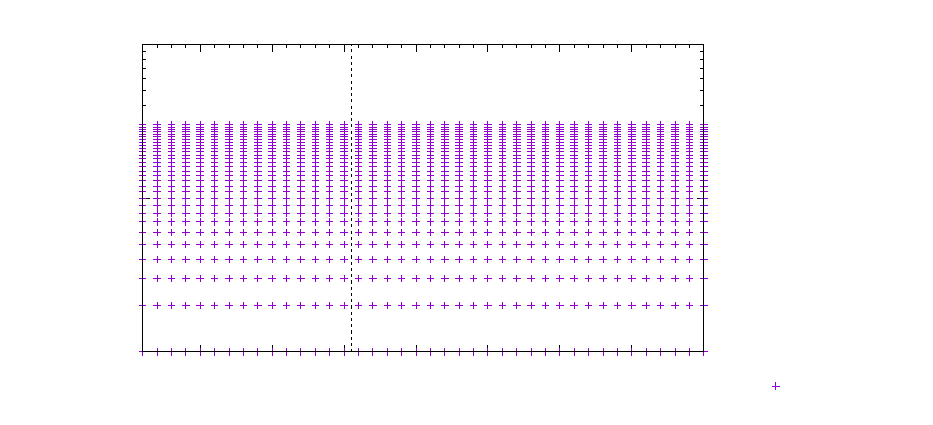
\includegraphics[width={432.00bp},height={188.60bp}]{../Plots/SCAMDWave/Diag/-2.5/plot}}%
    \gplfronttext
  \end{picture}%
\endgroup


  \caption{The expectation value of the c operators taking part into the gap as $\Delta_i = U_i\langle c_{i\uparrow}c_{i\downarrow}\rangle$. The  
  vertical periodic boundary condition makes each site on the same $x$-coordinate having the same value.
    We can then make an average on each of these columns and plot the result.}
\end{figure}
The superconducting gap lies around $0.01\cdot U$ and $0.16\cdot U$ for the range of selected chemical potentials. Further we observe a 
clear symmetry in the Cooper pairs distribution around the level $\mu =0$. The overlap of the Fermi surface with the s-wave seams
to be the same for $\pm\mu$ (see Fig. \ref{fig:Brillouin}). In fact if the accessible states are also found where the superconducting gap 
is defined, we expect the electrons to be more likely to bind into Cooper pairs.\\   
Further we observe some oscillations on the left and right sides that are well-defined over three to four sites towards the bulk. On these locations the sites have only three
neighbours, there are open boundaries, the rest is vacuum. One can see this lack of neighbours as impurities in the system. 
A first interpretation can be given by the Friedel oscillations \cite{Harrison1970}. The boundary disturbs the electron density and causes decreasing oscillations towards
the bulk. The Cooper-pairs being made of electrons, these oscillations are reflected in the gap as well. Another contribution to the oscillations
is the reflection of the quasiparticles.
These oscillations may be caused by Andrev bound states \cite{Bobkov_2024}, that may form because the quasiparticles are reflected at the boundary.
These can interfere with the Cooper pairs and cause the oscillations in the spacial representation of the energy gap.\\
\begin{figure}[H]
  \centering
  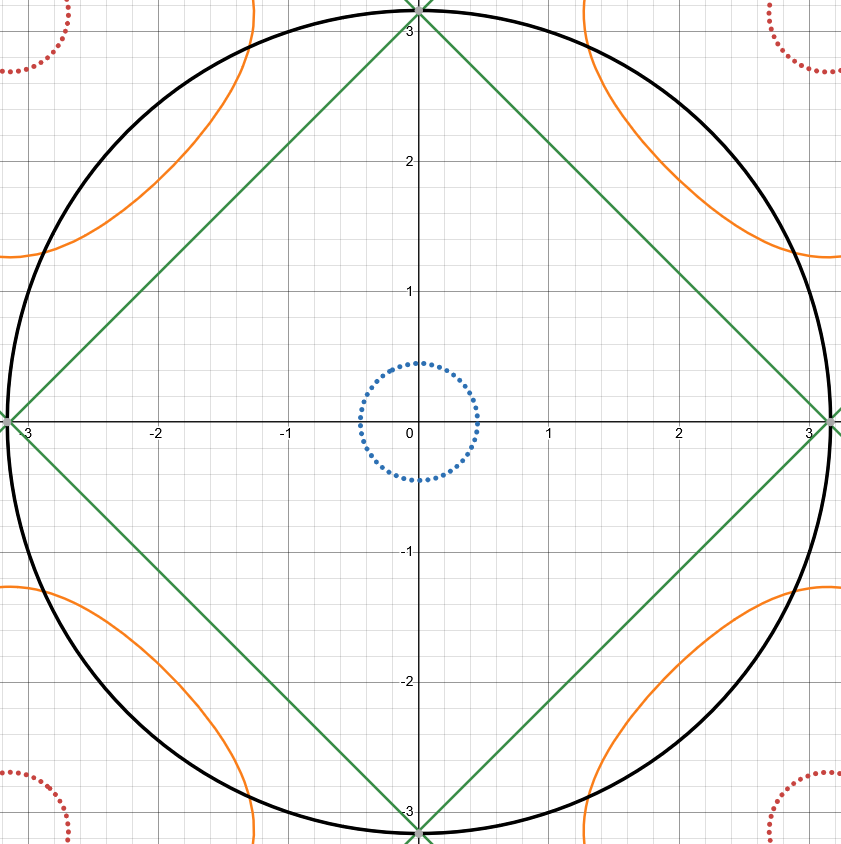
\includegraphics[width=0.45\textwidth]{Ressources/GapBrillouin.png}
  \caption{The first Brillouin zone with the Fermi surface for $\mu$ of \textcolor{Brillou1}{$\bm{-3.8}$}, \textcolor{Brillou2}{$\bm{0}$},
  \textcolor{Brillou3}{$\bm{1.4}$} and \textcolor{Brillou4}{$\bm{3.8}$}. The BCS gap is represented by the black circle. Its size is given such that 
  we can see that at a $\mu>0$ the states that can be found in the gap are less present until they vanish for a high $\mu$. For low $\mu$ there is
  not many states accessible to fill the gap as well. Figure made with Desmos.}
  \label{fig:Brillouin}
\end{figure}
In the simulation the size of the gap is such, that the Fermi surface 
covers the same area of the gap representation in reciprocal space for $\pm\mu$.
A maximum around $\mu=0$ is expected as the Fermi surface is the largest there.   

From this we can consider a proximity system by adding a different material on the right side of the superconductor. 
The most simple one is a normal metal (N) that has a hopping $t$ of $1$ in every direction.
Then we can replace it with an alternating hopping $t+m$ depending on a $\uparrow\uparrow$ interaction
and a $t-m$ depending on a $\downarrow\downarrow$ interaction. If this hopping takes place in every direction, this describes a ferromagnetic material (FM).
Making the sign of $m$ alternating if we have a hopping along the $x$ or the $y$ axis describes an altermagnet (AM).
Here we set $m=0.5$ and study different results for the chemical potential $\mu<0$ and compare the AM
with the others. $\ast$ represents a placeholder for the material a curve describes.\\
\begin{figure}[H]
  \centering
  % GNUPLOT: LaTeX picture with Postscript
\begingroup
  % Encoding inside the plot.  In the header of your document, this encoding
  % should to defined, e.g., by using
  % \usepackage[cp1252,<other encodings>]{inputenc}
  \inputencoding{cp1252}%
  \makeatletter
  \providecommand\color[2][]{%
    \GenericError{(gnuplot) \space\space\space\@spaces}{%
      Package color not loaded in conjunction with
      terminal option `colourtext'%
    }{See the gnuplot documentation for explanation.%
    }{Either use 'blacktext' in gnuplot or load the package
      color.sty in LaTeX.}%
    \renewcommand\color[2][]{}%
  }%
  \providecommand\includegraphics[2][]{%
    \GenericError{(gnuplot) \space\space\space\@spaces}{%
      Package graphicx or graphics not loaded%
    }{See the gnuplot documentation for explanation.%
    }{The gnuplot epslatex terminal needs graphicx.sty or graphics.sty.}%
    \renewcommand\includegraphics[2][]{}%
  }%
  \providecommand\rotatebox[2]{#2}%
  \@ifundefined{ifGPcolor}{%
    \newif\ifGPcolor
    \GPcolortrue
  }{}%
  \@ifundefined{ifGPblacktext}{%
    \newif\ifGPblacktext
    \GPblacktextfalse
  }{}%
  % define a \g@addto@macro without @ in the name:
  \let\gplgaddtomacro\g@addto@macro
  % define empty templates for all commands taking text:
  \gdef\gplbacktext{}%
  \gdef\gplfronttext{}%
  \makeatother
  \ifGPblacktext
    % no textcolor at all
    \def\colorrgb#1{}%
    \def\colorgray#1{}%
  \else
    % gray or color?
    \ifGPcolor
      \def\colorrgb#1{\color[rgb]{#1}}%
      \def\colorgray#1{\color[gray]{#1}}%
      \expandafter\def\csname LTw\endcsname{\color{white}}%
      \expandafter\def\csname LTb\endcsname{\color{black}}%
      \expandafter\def\csname LTa\endcsname{\color{black}}%
      \expandafter\def\csname LT0\endcsname{\color[rgb]{1,0,0}}%
      \expandafter\def\csname LT1\endcsname{\color[rgb]{0,1,0}}%
      \expandafter\def\csname LT2\endcsname{\color[rgb]{0,0,1}}%
      \expandafter\def\csname LT3\endcsname{\color[rgb]{1,0,1}}%
      \expandafter\def\csname LT4\endcsname{\color[rgb]{0,1,1}}%
      \expandafter\def\csname LT5\endcsname{\color[rgb]{1,1,0}}%
      \expandafter\def\csname LT6\endcsname{\color[rgb]{0,0,0}}%
      \expandafter\def\csname LT7\endcsname{\color[rgb]{1,0.3,0}}%
      \expandafter\def\csname LT8\endcsname{\color[rgb]{0.5,0.5,0.5}}%
    \else
      % gray
      \def\colorrgb#1{\color{black}}%
      \def\colorgray#1{\color[gray]{#1}}%
      \expandafter\def\csname LTw\endcsname{\color{white}}%
      \expandafter\def\csname LTb\endcsname{\color{black}}%
      \expandafter\def\csname LTa\endcsname{\color{black}}%
      \expandafter\def\csname LT0\endcsname{\color{black}}%
      \expandafter\def\csname LT1\endcsname{\color{black}}%
      \expandafter\def\csname LT2\endcsname{\color{black}}%
      \expandafter\def\csname LT3\endcsname{\color{black}}%
      \expandafter\def\csname LT4\endcsname{\color{black}}%
      \expandafter\def\csname LT5\endcsname{\color{black}}%
      \expandafter\def\csname LT6\endcsname{\color{black}}%
      \expandafter\def\csname LT7\endcsname{\color{black}}%
      \expandafter\def\csname LT8\endcsname{\color{black}}%
    \fi
  \fi
    \setlength{\unitlength}{0.0500bp}%
    \ifx\gptboxheight\undefined%
      \newlength{\gptboxheight}%
      \newlength{\gptboxwidth}%
      \newsavebox{\gptboxtext}%
    \fi%
    \setlength{\fboxrule}{0.5pt}%
    \setlength{\fboxsep}{1pt}%
    \definecolor{tbcol}{rgb}{1,1,1}%
\begin{picture}(8640.00,3772.00)%
    \gplgaddtomacro\gplbacktext{%
      \csname LTb\endcsname%%
      \put(946,542){\makebox(0,0){\scriptsize 1}}%
      \put(946,2018){\makebox(0,0){\scriptsize 10}}%
      \put(946,3493){\makebox(0,0){\scriptsize 100}}%
      \put(1762,410){\makebox(0,0){\scriptsize 5}}%
      \put(2453,410){\makebox(0,0){\scriptsize 10}}%
      \put(3143,410){\makebox(0,0){\scriptsize 15}}%
      \put(3834,410){\makebox(0,0){\scriptsize 20}}%
      \put(4524,410){\makebox(0,0){\scriptsize 25}}%
      \put(5215,410){\makebox(0,0){\scriptsize 30}}%
      \put(5905,410){\makebox(0,0){\scriptsize 35}}%
      \put(6596,410){\makebox(0,0){\scriptsize 40}}%
      \put(2557,3670){\makebox(0,0){\strut{}SC}}%
      \put(5250,3670){\makebox(0,0){\strut{}AM}}%
    }%
    \gplgaddtomacro\gplfronttext{%
      \csname LTb\endcsname%%
      \put(7715,212){\makebox(0,0)[l]{\strut{}\footnotesize -2.5}}%
      \csname LTb\endcsname%%
      \put(605,2017){\rotatebox{-270.00}{\makebox(0,0){\strut{}$\bm{|\langle c_{i\uparrow}c_{i\downarrow}\rangle|$}}}}%
      \put(3903,212){\makebox(0,0){\small\textbf{Lattice site $i$ in $\bm{e}_x$}}}%
    }%
    \gplbacktext
    \put(0,0){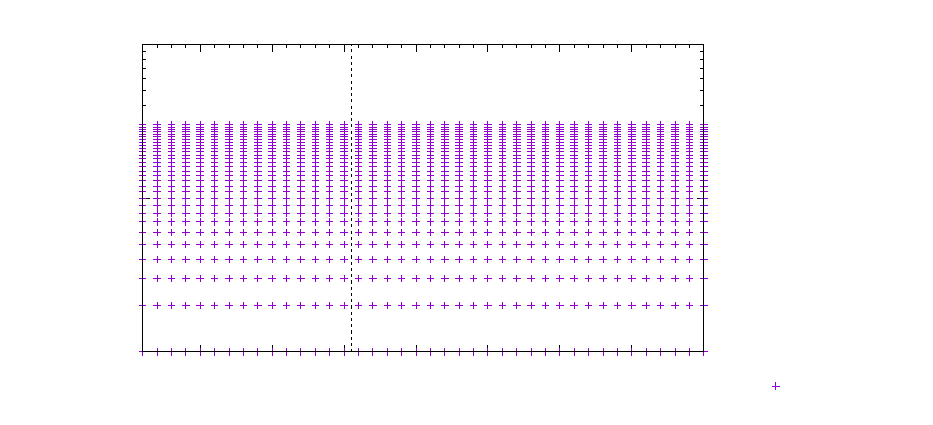
\includegraphics[width={432.00bp},height={188.60bp}]{../Plots/SCAMDWave/Diag/-2.5/plot}}%
    \gplfronttext
  \end{picture}%
\endgroup


  \caption{Evolution of the gap in the $x$ direction for a junction of SC-N, SC-FM and SC-AM at $\mu=-0.5$. Hopping $m=0.5$.}
  \label{fig:SC_START_Mu-0.5}
\end{figure}\begin{figure}[H]
  \centering
  % GNUPLOT: LaTeX picture with Postscript
\begingroup
  % Encoding inside the plot.  In the header of your document, this encoding
  % should to defined, e.g., by using
  % \usepackage[cp1252,<other encodings>]{inputenc}
  \inputencoding{cp1252}%
  \makeatletter
  \providecommand\color[2][]{%
    \GenericError{(gnuplot) \space\space\space\@spaces}{%
      Package color not loaded in conjunction with
      terminal option `colourtext'%
    }{See the gnuplot documentation for explanation.%
    }{Either use 'blacktext' in gnuplot or load the package
      color.sty in LaTeX.}%
    \renewcommand\color[2][]{}%
  }%
  \providecommand\includegraphics[2][]{%
    \GenericError{(gnuplot) \space\space\space\@spaces}{%
      Package graphicx or graphics not loaded%
    }{See the gnuplot documentation for explanation.%
    }{The gnuplot epslatex terminal needs graphicx.sty or graphics.sty.}%
    \renewcommand\includegraphics[2][]{}%
  }%
  \providecommand\rotatebox[2]{#2}%
  \@ifundefined{ifGPcolor}{%
    \newif\ifGPcolor
    \GPcolortrue
  }{}%
  \@ifundefined{ifGPblacktext}{%
    \newif\ifGPblacktext
    \GPblacktextfalse
  }{}%
  % define a \g@addto@macro without @ in the name:
  \let\gplgaddtomacro\g@addto@macro
  % define empty templates for all commands taking text:
  \gdef\gplbacktext{}%
  \gdef\gplfronttext{}%
  \makeatother
  \ifGPblacktext
    % no textcolor at all
    \def\colorrgb#1{}%
    \def\colorgray#1{}%
  \else
    % gray or color?
    \ifGPcolor
      \def\colorrgb#1{\color[rgb]{#1}}%
      \def\colorgray#1{\color[gray]{#1}}%
      \expandafter\def\csname LTw\endcsname{\color{white}}%
      \expandafter\def\csname LTb\endcsname{\color{black}}%
      \expandafter\def\csname LTa\endcsname{\color{black}}%
      \expandafter\def\csname LT0\endcsname{\color[rgb]{1,0,0}}%
      \expandafter\def\csname LT1\endcsname{\color[rgb]{0,1,0}}%
      \expandafter\def\csname LT2\endcsname{\color[rgb]{0,0,1}}%
      \expandafter\def\csname LT3\endcsname{\color[rgb]{1,0,1}}%
      \expandafter\def\csname LT4\endcsname{\color[rgb]{0,1,1}}%
      \expandafter\def\csname LT5\endcsname{\color[rgb]{1,1,0}}%
      \expandafter\def\csname LT6\endcsname{\color[rgb]{0,0,0}}%
      \expandafter\def\csname LT7\endcsname{\color[rgb]{1,0.3,0}}%
      \expandafter\def\csname LT8\endcsname{\color[rgb]{0.5,0.5,0.5}}%
    \else
      % gray
      \def\colorrgb#1{\color{black}}%
      \def\colorgray#1{\color[gray]{#1}}%
      \expandafter\def\csname LTw\endcsname{\color{white}}%
      \expandafter\def\csname LTb\endcsname{\color{black}}%
      \expandafter\def\csname LTa\endcsname{\color{black}}%
      \expandafter\def\csname LT0\endcsname{\color{black}}%
      \expandafter\def\csname LT1\endcsname{\color{black}}%
      \expandafter\def\csname LT2\endcsname{\color{black}}%
      \expandafter\def\csname LT3\endcsname{\color{black}}%
      \expandafter\def\csname LT4\endcsname{\color{black}}%
      \expandafter\def\csname LT5\endcsname{\color{black}}%
      \expandafter\def\csname LT6\endcsname{\color{black}}%
      \expandafter\def\csname LT7\endcsname{\color{black}}%
      \expandafter\def\csname LT8\endcsname{\color{black}}%
    \fi
  \fi
    \setlength{\unitlength}{0.0500bp}%
    \ifx\gptboxheight\undefined%
      \newlength{\gptboxheight}%
      \newlength{\gptboxwidth}%
      \newsavebox{\gptboxtext}%
    \fi%
    \setlength{\fboxrule}{0.5pt}%
    \setlength{\fboxsep}{1pt}%
    \definecolor{tbcol}{rgb}{1,1,1}%
\begin{picture}(8640.00,3772.00)%
    \gplgaddtomacro\gplbacktext{%
      \csname LTb\endcsname%%
      \put(946,542){\makebox(0,0){\scriptsize 1}}%
      \put(946,2018){\makebox(0,0){\scriptsize 10}}%
      \put(946,3493){\makebox(0,0){\scriptsize 100}}%
      \put(1762,410){\makebox(0,0){\scriptsize 5}}%
      \put(2453,410){\makebox(0,0){\scriptsize 10}}%
      \put(3143,410){\makebox(0,0){\scriptsize 15}}%
      \put(3834,410){\makebox(0,0){\scriptsize 20}}%
      \put(4524,410){\makebox(0,0){\scriptsize 25}}%
      \put(5215,410){\makebox(0,0){\scriptsize 30}}%
      \put(5905,410){\makebox(0,0){\scriptsize 35}}%
      \put(6596,410){\makebox(0,0){\scriptsize 40}}%
      \put(2557,3670){\makebox(0,0){\strut{}SC}}%
      \put(5250,3670){\makebox(0,0){\strut{}AM}}%
    }%
    \gplgaddtomacro\gplfronttext{%
      \csname LTb\endcsname%%
      \put(7715,212){\makebox(0,0)[l]{\strut{}\footnotesize -2.5}}%
      \csname LTb\endcsname%%
      \put(605,2017){\rotatebox{-270.00}{\makebox(0,0){\strut{}$\bm{|\langle c_{i\uparrow}c_{i\downarrow}\rangle|$}}}}%
      \put(3903,212){\makebox(0,0){\small\textbf{Lattice site $i$ in $\bm{e}_x$}}}%
    }%
    \gplbacktext
    \put(0,0){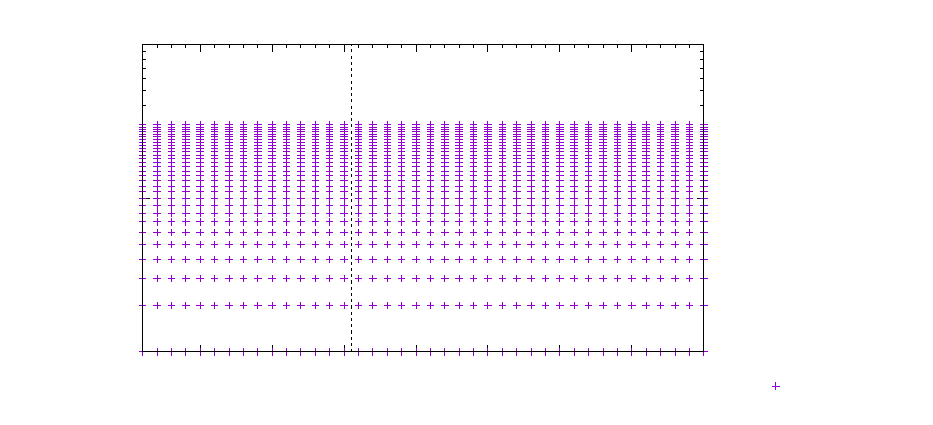
\includegraphics[width={432.00bp},height={188.60bp}]{../Plots/SCAMDWave/Diag/-2.5/plot}}%
    \gplfronttext
  \end{picture}%
\endgroup


  \caption{A junction of SC-N, SC-FM and SC-AM at $\mu=-1.5$, and a hopping $m=0.5$.}
  \label{fig:SC_START_Mu-1.5}
\end{figure}
\begin{figure}[H]
  \centering
  % GNUPLOT: LaTeX picture with Postscript
\begingroup
  % Encoding inside the plot.  In the header of your document, this encoding
  % should to defined, e.g., by using
  % \usepackage[cp1252,<other encodings>]{inputenc}
  \inputencoding{cp1252}%
  \makeatletter
  \providecommand\color[2][]{%
    \GenericError{(gnuplot) \space\space\space\@spaces}{%
      Package color not loaded in conjunction with
      terminal option `colourtext'%
    }{See the gnuplot documentation for explanation.%
    }{Either use 'blacktext' in gnuplot or load the package
      color.sty in LaTeX.}%
    \renewcommand\color[2][]{}%
  }%
  \providecommand\includegraphics[2][]{%
    \GenericError{(gnuplot) \space\space\space\@spaces}{%
      Package graphicx or graphics not loaded%
    }{See the gnuplot documentation for explanation.%
    }{The gnuplot epslatex terminal needs graphicx.sty or graphics.sty.}%
    \renewcommand\includegraphics[2][]{}%
  }%
  \providecommand\rotatebox[2]{#2}%
  \@ifundefined{ifGPcolor}{%
    \newif\ifGPcolor
    \GPcolortrue
  }{}%
  \@ifundefined{ifGPblacktext}{%
    \newif\ifGPblacktext
    \GPblacktextfalse
  }{}%
  % define a \g@addto@macro without @ in the name:
  \let\gplgaddtomacro\g@addto@macro
  % define empty templates for all commands taking text:
  \gdef\gplbacktext{}%
  \gdef\gplfronttext{}%
  \makeatother
  \ifGPblacktext
    % no textcolor at all
    \def\colorrgb#1{}%
    \def\colorgray#1{}%
  \else
    % gray or color?
    \ifGPcolor
      \def\colorrgb#1{\color[rgb]{#1}}%
      \def\colorgray#1{\color[gray]{#1}}%
      \expandafter\def\csname LTw\endcsname{\color{white}}%
      \expandafter\def\csname LTb\endcsname{\color{black}}%
      \expandafter\def\csname LTa\endcsname{\color{black}}%
      \expandafter\def\csname LT0\endcsname{\color[rgb]{1,0,0}}%
      \expandafter\def\csname LT1\endcsname{\color[rgb]{0,1,0}}%
      \expandafter\def\csname LT2\endcsname{\color[rgb]{0,0,1}}%
      \expandafter\def\csname LT3\endcsname{\color[rgb]{1,0,1}}%
      \expandafter\def\csname LT4\endcsname{\color[rgb]{0,1,1}}%
      \expandafter\def\csname LT5\endcsname{\color[rgb]{1,1,0}}%
      \expandafter\def\csname LT6\endcsname{\color[rgb]{0,0,0}}%
      \expandafter\def\csname LT7\endcsname{\color[rgb]{1,0.3,0}}%
      \expandafter\def\csname LT8\endcsname{\color[rgb]{0.5,0.5,0.5}}%
    \else
      % gray
      \def\colorrgb#1{\color{black}}%
      \def\colorgray#1{\color[gray]{#1}}%
      \expandafter\def\csname LTw\endcsname{\color{white}}%
      \expandafter\def\csname LTb\endcsname{\color{black}}%
      \expandafter\def\csname LTa\endcsname{\color{black}}%
      \expandafter\def\csname LT0\endcsname{\color{black}}%
      \expandafter\def\csname LT1\endcsname{\color{black}}%
      \expandafter\def\csname LT2\endcsname{\color{black}}%
      \expandafter\def\csname LT3\endcsname{\color{black}}%
      \expandafter\def\csname LT4\endcsname{\color{black}}%
      \expandafter\def\csname LT5\endcsname{\color{black}}%
      \expandafter\def\csname LT6\endcsname{\color{black}}%
      \expandafter\def\csname LT7\endcsname{\color{black}}%
      \expandafter\def\csname LT8\endcsname{\color{black}}%
    \fi
  \fi
    \setlength{\unitlength}{0.0500bp}%
    \ifx\gptboxheight\undefined%
      \newlength{\gptboxheight}%
      \newlength{\gptboxwidth}%
      \newsavebox{\gptboxtext}%
    \fi%
    \setlength{\fboxrule}{0.5pt}%
    \setlength{\fboxsep}{1pt}%
    \definecolor{tbcol}{rgb}{1,1,1}%
\begin{picture}(8640.00,3772.00)%
    \gplgaddtomacro\gplbacktext{%
      \csname LTb\endcsname%%
      \put(946,542){\makebox(0,0){\scriptsize 1}}%
      \put(946,2018){\makebox(0,0){\scriptsize 10}}%
      \put(946,3493){\makebox(0,0){\scriptsize 100}}%
      \put(1762,410){\makebox(0,0){\scriptsize 5}}%
      \put(2453,410){\makebox(0,0){\scriptsize 10}}%
      \put(3143,410){\makebox(0,0){\scriptsize 15}}%
      \put(3834,410){\makebox(0,0){\scriptsize 20}}%
      \put(4524,410){\makebox(0,0){\scriptsize 25}}%
      \put(5215,410){\makebox(0,0){\scriptsize 30}}%
      \put(5905,410){\makebox(0,0){\scriptsize 35}}%
      \put(6596,410){\makebox(0,0){\scriptsize 40}}%
      \put(2557,3670){\makebox(0,0){\strut{}SC}}%
      \put(5250,3670){\makebox(0,0){\strut{}AM}}%
    }%
    \gplgaddtomacro\gplfronttext{%
      \csname LTb\endcsname%%
      \put(7715,212){\makebox(0,0)[l]{\strut{}\footnotesize -2.5}}%
      \csname LTb\endcsname%%
      \put(605,2017){\rotatebox{-270.00}{\makebox(0,0){\strut{}$\bm{|\langle c_{i\uparrow}c_{i\downarrow}\rangle|$}}}}%
      \put(3903,212){\makebox(0,0){\small\textbf{Lattice site $i$ in $\bm{e}_x$}}}%
    }%
    \gplbacktext
    \put(0,0){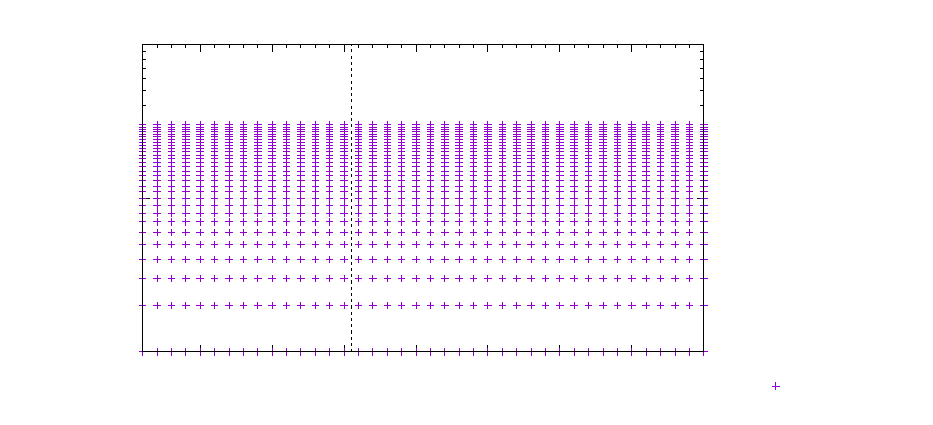
\includegraphics[width={432.00bp},height={188.60bp}]{../Plots/SCAMDWave/Diag/-2.5/plot}}%
    \gplfronttext
  \end{picture}%
\endgroup


  \caption{A junction of SC-N, SC-FM and SC-AM at $\mu=-2.5$, and a hopping $m=0.5$.}
    \label{fig:SC_START_Mu-2.5}
\end{figure}
We first take a look at the superconductor (SC). Inside it the gap is not be the same for $\mu=-0.5,-1.5$
and settles around $0.1\cdot U$. Most likely the increase of the Fermi surface do not give an additional contribution to the gap.
The gap is however one order of magnitude smaller for $\mu=-2.5$. Here the withdrawal of the Fermi surface is more relevant and the 
gap becomes smaller.\\
We have a clear decay of the gap after entering the normal metal (N). At this point 
study that were already made tend to have an exponential decay of the gap \cite{Mjos2019}. Having a logarithmic scale we would
except a more straight line, but this is still a reasonable exponential decay. A way to approach the line would be to increase the 
resolution of the lattice, as well as simulating a more squared one. This decay makes the expectation value having an order of 
magnitude of difference from one side to the other of the N. For the smallest $\mu$ we see that the decay is weaker, the gap lost
half of its amplitude after crossing the N. Further we see that both the FM and the AM add some oscillations in the decay. \\

The ferromagnet follows closely the normal metal for $\mu=-0.5,-1.5$. It is interesting to note a real nice exponential
decay when having a chemical potential of $-2.5$ modulated by oscillations. We observe about the same number of oscillations and about of
the same amplitude in these three cases. In the AM the initial decay is stronger in the sites near the 
interface than in the FM. Then the decay seams to follow the FM. We observe about the same number of oscillations in the FM and the AM.
For $\mu=-0.5$ we observe a clean line in the first four sites of the AM. Then we have oscillations and the Cooper-pairs are more present
than expected regarding the initial decay. The reason might be that the first oscillation combined with the initial decay make the line
reach it's second-deepest point (around $10^{-4}$) and therefore everything looks more flat.

In the AM the oscillation amplitude increases with a decreasing $|\mu|$.
We observe nearly two orders of magnitude in their amplitude for $\mu=-0.5$ compared to one order of magnitude for $\mu=-2.5$.
We tried to simulate these for a $\mu=-3.5$ but the algorithm  converge to values that are numerically zero everywhere ($10^{-16}$).
It looks like the Fermi-surface is too small and there is a lack of electrons to build the Cooper pairs.\\
 
These oscillations are more likely due to the fact that we have a spin-dependent hopping. In fact, we have the same behaviour for the AM
and the FM, but not in the N. As a result of the spin-splitted Fermi surfaces the electrons in the Cooper pairs have different momenta.
This phenomenon causes the superconductivity correlation in the FM to oscillate \cite{Jong1995}. A similar behaviour happens inside the AM.

This dynamic influences the gap, and the different components of the gap interfere with each other resulting
periodically in especially low values. We see that the direction-dependence of the altermagnetic hopping causes a weaker gap and 
oscillations of bigger amplitudes. Traces of Friedel oscillations and quasiparticles' reflections are still visible, especially in the non-SC materials.\\

We now want to simulate the behaviour of the s-wave superconductivity on a diagonal interface. We focus on three different values of $\mu<0$.  
The diagonal is build by rotating the interface by $45^{\circ}$ around the centre of the lattice. The upper-part, regarding the $y$-axis is the SC
and the lower one the AM. We set $m=0.5$.
\begin{figure}[H]
    \centering
    % GNUPLOT: LaTeX picture with Postscript
\begingroup
  % Encoding inside the plot.  In the header of your document, this encoding
  % should to defined, e.g., by using
  % \usepackage[cp1252,<other encodings>]{inputenc}
  \inputencoding{cp1252}%
  \makeatletter
  \providecommand\color[2][]{%
    \GenericError{(gnuplot) \space\space\space\@spaces}{%
      Package color not loaded in conjunction with
      terminal option `colourtext'%
    }{See the gnuplot documentation for explanation.%
    }{Either use 'blacktext' in gnuplot or load the package
      color.sty in LaTeX.}%
    \renewcommand\color[2][]{}%
  }%
  \providecommand\includegraphics[2][]{%
    \GenericError{(gnuplot) \space\space\space\@spaces}{%
      Package graphicx or graphics not loaded%
    }{See the gnuplot documentation for explanation.%
    }{The gnuplot epslatex terminal needs graphicx.sty or graphics.sty.}%
    \renewcommand\includegraphics[2][]{}%
  }%
  \providecommand\rotatebox[2]{#2}%
  \@ifundefined{ifGPcolor}{%
    \newif\ifGPcolor
    \GPcolortrue
  }{}%
  \@ifundefined{ifGPblacktext}{%
    \newif\ifGPblacktext
    \GPblacktextfalse
  }{}%
  % define a \g@addto@macro without @ in the name:
  \let\gplgaddtomacro\g@addto@macro
  % define empty templates for all commands taking text:
  \gdef\gplbacktext{}%
  \gdef\gplfronttext{}%
  \makeatother
  \ifGPblacktext
    % no textcolor at all
    \def\colorrgb#1{}%
    \def\colorgray#1{}%
  \else
    % gray or color?
    \ifGPcolor
      \def\colorrgb#1{\color[rgb]{#1}}%
      \def\colorgray#1{\color[gray]{#1}}%
      \expandafter\def\csname LTw\endcsname{\color{white}}%
      \expandafter\def\csname LTb\endcsname{\color{black}}%
      \expandafter\def\csname LTa\endcsname{\color{black}}%
      \expandafter\def\csname LT0\endcsname{\color[rgb]{1,0,0}}%
      \expandafter\def\csname LT1\endcsname{\color[rgb]{0,1,0}}%
      \expandafter\def\csname LT2\endcsname{\color[rgb]{0,0,1}}%
      \expandafter\def\csname LT3\endcsname{\color[rgb]{1,0,1}}%
      \expandafter\def\csname LT4\endcsname{\color[rgb]{0,1,1}}%
      \expandafter\def\csname LT5\endcsname{\color[rgb]{1,1,0}}%
      \expandafter\def\csname LT6\endcsname{\color[rgb]{0,0,0}}%
      \expandafter\def\csname LT7\endcsname{\color[rgb]{1,0.3,0}}%
      \expandafter\def\csname LT8\endcsname{\color[rgb]{0.5,0.5,0.5}}%
    \else
      % gray
      \def\colorrgb#1{\color{black}}%
      \def\colorgray#1{\color[gray]{#1}}%
      \expandafter\def\csname LTw\endcsname{\color{white}}%
      \expandafter\def\csname LTb\endcsname{\color{black}}%
      \expandafter\def\csname LTa\endcsname{\color{black}}%
      \expandafter\def\csname LT0\endcsname{\color{black}}%
      \expandafter\def\csname LT1\endcsname{\color{black}}%
      \expandafter\def\csname LT2\endcsname{\color{black}}%
      \expandafter\def\csname LT3\endcsname{\color{black}}%
      \expandafter\def\csname LT4\endcsname{\color{black}}%
      \expandafter\def\csname LT5\endcsname{\color{black}}%
      \expandafter\def\csname LT6\endcsname{\color{black}}%
      \expandafter\def\csname LT7\endcsname{\color{black}}%
      \expandafter\def\csname LT8\endcsname{\color{black}}%
    \fi
  \fi
    \setlength{\unitlength}{0.0500bp}%
    \ifx\gptboxheight\undefined%
      \newlength{\gptboxheight}%
      \newlength{\gptboxwidth}%
      \newsavebox{\gptboxtext}%
    \fi%
    \setlength{\fboxrule}{0.5pt}%
    \setlength{\fboxsep}{1pt}%
    \definecolor{tbcol}{rgb}{1,1,1}%
\begin{picture}(8640.00,3772.00)%
    \gplgaddtomacro\gplbacktext{%
      \csname LTb\endcsname%%
      \put(946,542){\makebox(0,0){\scriptsize 1}}%
      \put(946,2018){\makebox(0,0){\scriptsize 10}}%
      \put(946,3493){\makebox(0,0){\scriptsize 100}}%
      \put(1762,410){\makebox(0,0){\scriptsize 5}}%
      \put(2453,410){\makebox(0,0){\scriptsize 10}}%
      \put(3143,410){\makebox(0,0){\scriptsize 15}}%
      \put(3834,410){\makebox(0,0){\scriptsize 20}}%
      \put(4524,410){\makebox(0,0){\scriptsize 25}}%
      \put(5215,410){\makebox(0,0){\scriptsize 30}}%
      \put(5905,410){\makebox(0,0){\scriptsize 35}}%
      \put(6596,410){\makebox(0,0){\scriptsize 40}}%
      \put(2557,3670){\makebox(0,0){\strut{}SC}}%
      \put(5250,3670){\makebox(0,0){\strut{}AM}}%
    }%
    \gplgaddtomacro\gplfronttext{%
      \csname LTb\endcsname%%
      \put(7715,212){\makebox(0,0)[l]{\strut{}\footnotesize -2.5}}%
      \csname LTb\endcsname%%
      \put(605,2017){\rotatebox{-270.00}{\makebox(0,0){\strut{}$\bm{|\langle c_{i\uparrow}c_{i\downarrow}\rangle|$}}}}%
      \put(3903,212){\makebox(0,0){\small\textbf{Lattice site $i$ in $\bm{e}_x$}}}%
    }%
    \gplbacktext
    \put(0,0){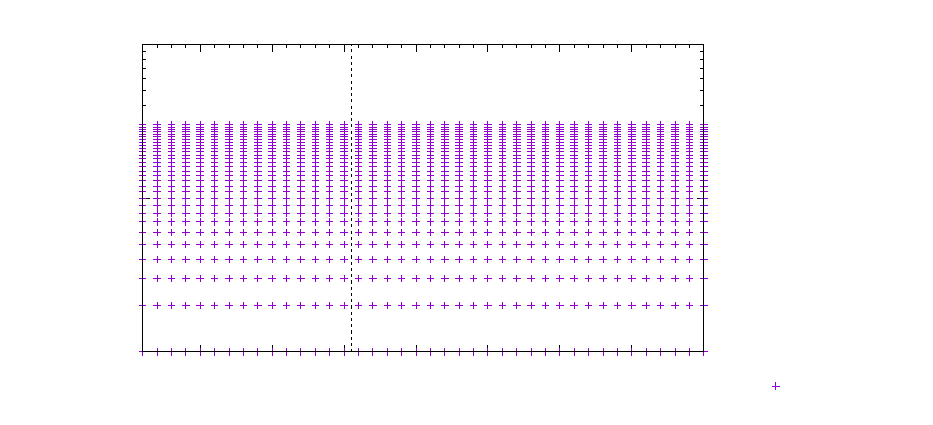
\includegraphics[width={432.00bp},height={188.60bp}]{../Plots/SCAMDWave/Diag/-2.5/plot}}%
    \gplfronttext
  \end{picture}%
\endgroup


    \caption{Diagonal interface of a SC and an AM at $\mu = -2.5$.}
\end{figure}
\begin{figure}[H]
    \centering
    % GNUPLOT: LaTeX picture with Postscript
\begingroup
  % Encoding inside the plot.  In the header of your document, this encoding
  % should to defined, e.g., by using
  % \usepackage[cp1252,<other encodings>]{inputenc}
  \inputencoding{cp1252}%
  \makeatletter
  \providecommand\color[2][]{%
    \GenericError{(gnuplot) \space\space\space\@spaces}{%
      Package color not loaded in conjunction with
      terminal option `colourtext'%
    }{See the gnuplot documentation for explanation.%
    }{Either use 'blacktext' in gnuplot or load the package
      color.sty in LaTeX.}%
    \renewcommand\color[2][]{}%
  }%
  \providecommand\includegraphics[2][]{%
    \GenericError{(gnuplot) \space\space\space\@spaces}{%
      Package graphicx or graphics not loaded%
    }{See the gnuplot documentation for explanation.%
    }{The gnuplot epslatex terminal needs graphicx.sty or graphics.sty.}%
    \renewcommand\includegraphics[2][]{}%
  }%
  \providecommand\rotatebox[2]{#2}%
  \@ifundefined{ifGPcolor}{%
    \newif\ifGPcolor
    \GPcolortrue
  }{}%
  \@ifundefined{ifGPblacktext}{%
    \newif\ifGPblacktext
    \GPblacktextfalse
  }{}%
  % define a \g@addto@macro without @ in the name:
  \let\gplgaddtomacro\g@addto@macro
  % define empty templates for all commands taking text:
  \gdef\gplbacktext{}%
  \gdef\gplfronttext{}%
  \makeatother
  \ifGPblacktext
    % no textcolor at all
    \def\colorrgb#1{}%
    \def\colorgray#1{}%
  \else
    % gray or color?
    \ifGPcolor
      \def\colorrgb#1{\color[rgb]{#1}}%
      \def\colorgray#1{\color[gray]{#1}}%
      \expandafter\def\csname LTw\endcsname{\color{white}}%
      \expandafter\def\csname LTb\endcsname{\color{black}}%
      \expandafter\def\csname LTa\endcsname{\color{black}}%
      \expandafter\def\csname LT0\endcsname{\color[rgb]{1,0,0}}%
      \expandafter\def\csname LT1\endcsname{\color[rgb]{0,1,0}}%
      \expandafter\def\csname LT2\endcsname{\color[rgb]{0,0,1}}%
      \expandafter\def\csname LT3\endcsname{\color[rgb]{1,0,1}}%
      \expandafter\def\csname LT4\endcsname{\color[rgb]{0,1,1}}%
      \expandafter\def\csname LT5\endcsname{\color[rgb]{1,1,0}}%
      \expandafter\def\csname LT6\endcsname{\color[rgb]{0,0,0}}%
      \expandafter\def\csname LT7\endcsname{\color[rgb]{1,0.3,0}}%
      \expandafter\def\csname LT8\endcsname{\color[rgb]{0.5,0.5,0.5}}%
    \else
      % gray
      \def\colorrgb#1{\color{black}}%
      \def\colorgray#1{\color[gray]{#1}}%
      \expandafter\def\csname LTw\endcsname{\color{white}}%
      \expandafter\def\csname LTb\endcsname{\color{black}}%
      \expandafter\def\csname LTa\endcsname{\color{black}}%
      \expandafter\def\csname LT0\endcsname{\color{black}}%
      \expandafter\def\csname LT1\endcsname{\color{black}}%
      \expandafter\def\csname LT2\endcsname{\color{black}}%
      \expandafter\def\csname LT3\endcsname{\color{black}}%
      \expandafter\def\csname LT4\endcsname{\color{black}}%
      \expandafter\def\csname LT5\endcsname{\color{black}}%
      \expandafter\def\csname LT6\endcsname{\color{black}}%
      \expandafter\def\csname LT7\endcsname{\color{black}}%
      \expandafter\def\csname LT8\endcsname{\color{black}}%
    \fi
  \fi
    \setlength{\unitlength}{0.0500bp}%
    \ifx\gptboxheight\undefined%
      \newlength{\gptboxheight}%
      \newlength{\gptboxwidth}%
      \newsavebox{\gptboxtext}%
    \fi%
    \setlength{\fboxrule}{0.5pt}%
    \setlength{\fboxsep}{1pt}%
    \definecolor{tbcol}{rgb}{1,1,1}%
\begin{picture}(8640.00,3772.00)%
    \gplgaddtomacro\gplbacktext{%
      \csname LTb\endcsname%%
      \put(946,542){\makebox(0,0){\scriptsize 1}}%
      \put(946,2018){\makebox(0,0){\scriptsize 10}}%
      \put(946,3493){\makebox(0,0){\scriptsize 100}}%
      \put(1762,410){\makebox(0,0){\scriptsize 5}}%
      \put(2453,410){\makebox(0,0){\scriptsize 10}}%
      \put(3143,410){\makebox(0,0){\scriptsize 15}}%
      \put(3834,410){\makebox(0,0){\scriptsize 20}}%
      \put(4524,410){\makebox(0,0){\scriptsize 25}}%
      \put(5215,410){\makebox(0,0){\scriptsize 30}}%
      \put(5905,410){\makebox(0,0){\scriptsize 35}}%
      \put(6596,410){\makebox(0,0){\scriptsize 40}}%
      \put(2557,3670){\makebox(0,0){\strut{}SC}}%
      \put(5250,3670){\makebox(0,0){\strut{}AM}}%
    }%
    \gplgaddtomacro\gplfronttext{%
      \csname LTb\endcsname%%
      \put(7715,212){\makebox(0,0)[l]{\strut{}\footnotesize -2.5}}%
      \csname LTb\endcsname%%
      \put(605,2017){\rotatebox{-270.00}{\makebox(0,0){\strut{}$\bm{|\langle c_{i\uparrow}c_{i\downarrow}\rangle|$}}}}%
      \put(3903,212){\makebox(0,0){\small\textbf{Lattice site $i$ in $\bm{e}_x$}}}%
    }%
    \gplbacktext
    \put(0,0){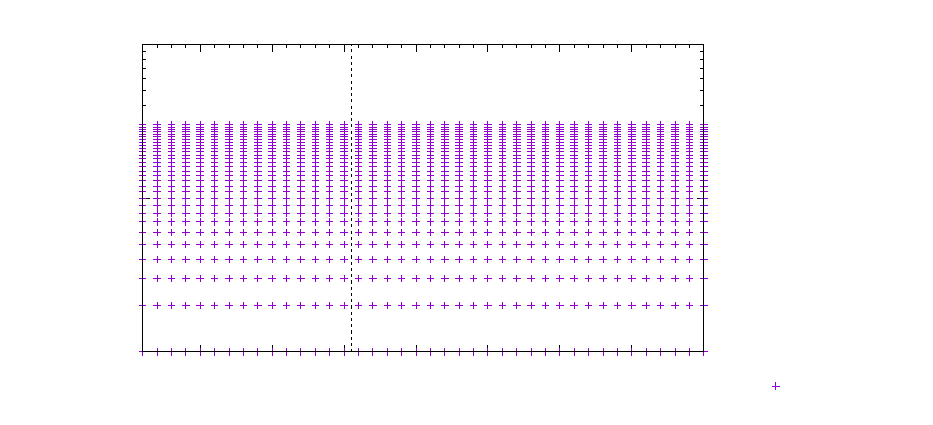
\includegraphics[width={432.00bp},height={188.60bp}]{../Plots/SCAMDWave/Diag/-2.5/plot}}%
    \gplfronttext
  \end{picture}%
\endgroup


    \caption{Diagonal interface of a SC and an AM at $\mu = -1.5$.}
\end{figure}
\begin{figure}[H]
    \centering
    % GNUPLOT: LaTeX picture with Postscript
\begingroup
  % Encoding inside the plot.  In the header of your document, this encoding
  % should to defined, e.g., by using
  % \usepackage[cp1252,<other encodings>]{inputenc}
  \inputencoding{cp1252}%
  \makeatletter
  \providecommand\color[2][]{%
    \GenericError{(gnuplot) \space\space\space\@spaces}{%
      Package color not loaded in conjunction with
      terminal option `colourtext'%
    }{See the gnuplot documentation for explanation.%
    }{Either use 'blacktext' in gnuplot or load the package
      color.sty in LaTeX.}%
    \renewcommand\color[2][]{}%
  }%
  \providecommand\includegraphics[2][]{%
    \GenericError{(gnuplot) \space\space\space\@spaces}{%
      Package graphicx or graphics not loaded%
    }{See the gnuplot documentation for explanation.%
    }{The gnuplot epslatex terminal needs graphicx.sty or graphics.sty.}%
    \renewcommand\includegraphics[2][]{}%
  }%
  \providecommand\rotatebox[2]{#2}%
  \@ifundefined{ifGPcolor}{%
    \newif\ifGPcolor
    \GPcolortrue
  }{}%
  \@ifundefined{ifGPblacktext}{%
    \newif\ifGPblacktext
    \GPblacktextfalse
  }{}%
  % define a \g@addto@macro without @ in the name:
  \let\gplgaddtomacro\g@addto@macro
  % define empty templates for all commands taking text:
  \gdef\gplbacktext{}%
  \gdef\gplfronttext{}%
  \makeatother
  \ifGPblacktext
    % no textcolor at all
    \def\colorrgb#1{}%
    \def\colorgray#1{}%
  \else
    % gray or color?
    \ifGPcolor
      \def\colorrgb#1{\color[rgb]{#1}}%
      \def\colorgray#1{\color[gray]{#1}}%
      \expandafter\def\csname LTw\endcsname{\color{white}}%
      \expandafter\def\csname LTb\endcsname{\color{black}}%
      \expandafter\def\csname LTa\endcsname{\color{black}}%
      \expandafter\def\csname LT0\endcsname{\color[rgb]{1,0,0}}%
      \expandafter\def\csname LT1\endcsname{\color[rgb]{0,1,0}}%
      \expandafter\def\csname LT2\endcsname{\color[rgb]{0,0,1}}%
      \expandafter\def\csname LT3\endcsname{\color[rgb]{1,0,1}}%
      \expandafter\def\csname LT4\endcsname{\color[rgb]{0,1,1}}%
      \expandafter\def\csname LT5\endcsname{\color[rgb]{1,1,0}}%
      \expandafter\def\csname LT6\endcsname{\color[rgb]{0,0,0}}%
      \expandafter\def\csname LT7\endcsname{\color[rgb]{1,0.3,0}}%
      \expandafter\def\csname LT8\endcsname{\color[rgb]{0.5,0.5,0.5}}%
    \else
      % gray
      \def\colorrgb#1{\color{black}}%
      \def\colorgray#1{\color[gray]{#1}}%
      \expandafter\def\csname LTw\endcsname{\color{white}}%
      \expandafter\def\csname LTb\endcsname{\color{black}}%
      \expandafter\def\csname LTa\endcsname{\color{black}}%
      \expandafter\def\csname LT0\endcsname{\color{black}}%
      \expandafter\def\csname LT1\endcsname{\color{black}}%
      \expandafter\def\csname LT2\endcsname{\color{black}}%
      \expandafter\def\csname LT3\endcsname{\color{black}}%
      \expandafter\def\csname LT4\endcsname{\color{black}}%
      \expandafter\def\csname LT5\endcsname{\color{black}}%
      \expandafter\def\csname LT6\endcsname{\color{black}}%
      \expandafter\def\csname LT7\endcsname{\color{black}}%
      \expandafter\def\csname LT8\endcsname{\color{black}}%
    \fi
  \fi
    \setlength{\unitlength}{0.0500bp}%
    \ifx\gptboxheight\undefined%
      \newlength{\gptboxheight}%
      \newlength{\gptboxwidth}%
      \newsavebox{\gptboxtext}%
    \fi%
    \setlength{\fboxrule}{0.5pt}%
    \setlength{\fboxsep}{1pt}%
    \definecolor{tbcol}{rgb}{1,1,1}%
\begin{picture}(8640.00,3772.00)%
    \gplgaddtomacro\gplbacktext{%
      \csname LTb\endcsname%%
      \put(946,542){\makebox(0,0){\scriptsize 1}}%
      \put(946,2018){\makebox(0,0){\scriptsize 10}}%
      \put(946,3493){\makebox(0,0){\scriptsize 100}}%
      \put(1762,410){\makebox(0,0){\scriptsize 5}}%
      \put(2453,410){\makebox(0,0){\scriptsize 10}}%
      \put(3143,410){\makebox(0,0){\scriptsize 15}}%
      \put(3834,410){\makebox(0,0){\scriptsize 20}}%
      \put(4524,410){\makebox(0,0){\scriptsize 25}}%
      \put(5215,410){\makebox(0,0){\scriptsize 30}}%
      \put(5905,410){\makebox(0,0){\scriptsize 35}}%
      \put(6596,410){\makebox(0,0){\scriptsize 40}}%
      \put(2557,3670){\makebox(0,0){\strut{}SC}}%
      \put(5250,3670){\makebox(0,0){\strut{}AM}}%
    }%
    \gplgaddtomacro\gplfronttext{%
      \csname LTb\endcsname%%
      \put(7715,212){\makebox(0,0)[l]{\strut{}\footnotesize -2.5}}%
      \csname LTb\endcsname%%
      \put(605,2017){\rotatebox{-270.00}{\makebox(0,0){\strut{}$\bm{|\langle c_{i\uparrow}c_{i\downarrow}\rangle|$}}}}%
      \put(3903,212){\makebox(0,0){\small\textbf{Lattice site $i$ in $\bm{e}_x$}}}%
    }%
    \gplbacktext
    \put(0,0){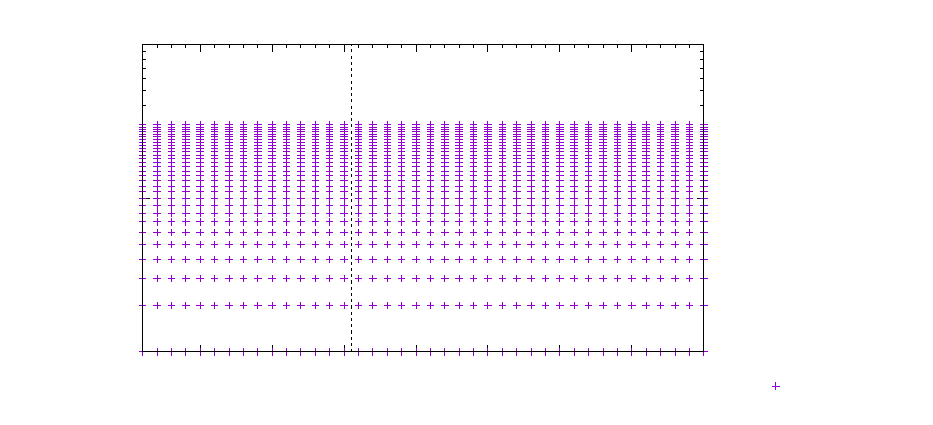
\includegraphics[width={432.00bp},height={188.60bp}]{../Plots/SCAMDWave/Diag/-2.5/plot}}%
    \gplfronttext
  \end{picture}%
\endgroup


    \caption{Diagonal interface of a SC and an AM at $\mu = -0.5$.}
\end{figure}
The superconductivity fills uniformly the superconductor. Consistently with the previous observations 
(Fig. \ref{fig:SC_START_Mu-0.5}, \ref{fig:SC_START_Mu-1.5} and \ref{fig:SC_START_Mu-2.5}) its magnitude grows, while $|\mu|$ get closer to zero.
 

Once again the oscillating exponential decay is present. We count up to eight oscillations for the three cases of study, whose
frequency is around three sites in all configurations. The oscillations take only place along the $x$ axis but the exponential decay
seams to point along the normal of the interface, making the (40,0) region the less populated in Cooper pairs.
The lower the $|\mu|$, the less noise we observe in the plots. Similarly to the straight interface the decay is strong in the begging
and then slows down when approaching the farthest regions from the interface.\\

If we try to find the line for a given $y$ that has the same site length in the AM in the straight interface case, we can pick one the at $y=15$.
There we count the same number of oscillations in the AM than in the straight interface case. In fact at $y=1$ we can see that the AM was
extended and at $y=30$ we can see that the AM was shortened. This gives the room to more oscillations to happen in the first case,
and less in the second one. The profile of the oscillations \textit{along the $x$ axis} is the same as in the straight interface case. \\

As before, this increase in Cooper pairs formation with decreasing $|\mu|$ is due to the shape of the Fermi surface.
Considering only the SC, we see an increase of an order of magnitude between $\mu=-2.5$ and $\mu=-1.5$. On the other hand we only count
a doubling of the Cooper pairs from $\mu=-1.5$ and $\mu=-0.5$.
As before the majority of the newly accessible states provided by $\mu=-0.5$ are outside the s-wave range.
This yields to a smaller increase in the number of Cooper pairs when compared to the first case.


We know that the Cooper pairs leak from the SC. We can reasonably say that they can leak in every direction from a site on the interface.
Due to interferences between them, we can expect to have a net diffusion along the normal of the interface. By doing so the leaking that we see
should be considered along the $(1,-1)$ axis: The leaking goes through the oscillations along the normal. This results in more spread
oscillations than in the straight interface case for the same travel length.

\begin{figure}[H]
  \centering
  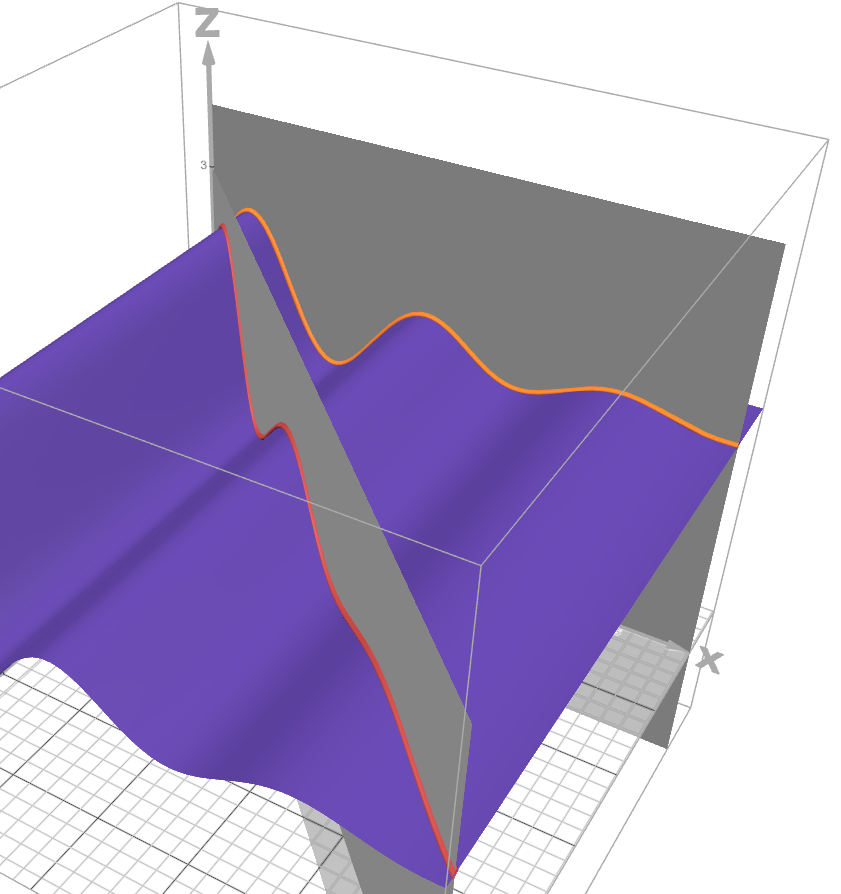
\includegraphics[width=0.5\textwidth]{Ressources/CooperPairsOrient.PNG}
  \caption{An arbitrary oscillating exponential decay in the $x$-direction. Going these oscillations along $x$ or along the diagonal $(1,-1)$ axis results in different
  experienced oscillations for the same travel length. Plot made with Desmos.}
\end{figure}
Towards simulating the Josephon junction we can represent the current in the superconductor: \rem{Here OBC are used, will be replaced by vertical ones
to agree with the rest of the study.} 
We know \rem{(additional small section needed in the theory)} that the current is proportional to the phase gradient of the superconducting gap.
We can experimentally apply a voltage difference between the two sides of the superconductor to induce a phase gradient \rem{source}.
To simulate this we will hold the phase fixed on the sides maintaining a difference of $117^{\circ}$ between the two sides.
We start this gradient at two different angles $\varphi_0 = -2\pi/3$ and $\varphi_0 = \pi/3$ on the left side.
\begin{figure}[H]
    % GNUPLOT: LaTeX picture with Postscript
\begingroup
  % Encoding inside the plot.  In the header of your document, this encoding
  % should to defined, e.g., by using
  % \usepackage[cp1252,<other encodings>]{inputenc}
  \inputencoding{cp1252}%
  \makeatletter
  \providecommand\color[2][]{%
    \GenericError{(gnuplot) \space\space\space\@spaces}{%
      Package color not loaded in conjunction with
      terminal option `colourtext'%
    }{See the gnuplot documentation for explanation.%
    }{Either use 'blacktext' in gnuplot or load the package
      color.sty in LaTeX.}%
    \renewcommand\color[2][]{}%
  }%
  \providecommand\includegraphics[2][]{%
    \GenericError{(gnuplot) \space\space\space\@spaces}{%
      Package graphicx or graphics not loaded%
    }{See the gnuplot documentation for explanation.%
    }{The gnuplot epslatex terminal needs graphicx.sty or graphics.sty.}%
    \renewcommand\includegraphics[2][]{}%
  }%
  \providecommand\rotatebox[2]{#2}%
  \@ifundefined{ifGPcolor}{%
    \newif\ifGPcolor
    \GPcolortrue
  }{}%
  \@ifundefined{ifGPblacktext}{%
    \newif\ifGPblacktext
    \GPblacktextfalse
  }{}%
  % define a \g@addto@macro without @ in the name:
  \let\gplgaddtomacro\g@addto@macro
  % define empty templates for all commands taking text:
  \gdef\gplbacktext{}%
  \gdef\gplfronttext{}%
  \makeatother
  \ifGPblacktext
    % no textcolor at all
    \def\colorrgb#1{}%
    \def\colorgray#1{}%
  \else
    % gray or color?
    \ifGPcolor
      \def\colorrgb#1{\color[rgb]{#1}}%
      \def\colorgray#1{\color[gray]{#1}}%
      \expandafter\def\csname LTw\endcsname{\color{white}}%
      \expandafter\def\csname LTb\endcsname{\color{black}}%
      \expandafter\def\csname LTa\endcsname{\color{black}}%
      \expandafter\def\csname LT0\endcsname{\color[rgb]{1,0,0}}%
      \expandafter\def\csname LT1\endcsname{\color[rgb]{0,1,0}}%
      \expandafter\def\csname LT2\endcsname{\color[rgb]{0,0,1}}%
      \expandafter\def\csname LT3\endcsname{\color[rgb]{1,0,1}}%
      \expandafter\def\csname LT4\endcsname{\color[rgb]{0,1,1}}%
      \expandafter\def\csname LT5\endcsname{\color[rgb]{1,1,0}}%
      \expandafter\def\csname LT6\endcsname{\color[rgb]{0,0,0}}%
      \expandafter\def\csname LT7\endcsname{\color[rgb]{1,0.3,0}}%
      \expandafter\def\csname LT8\endcsname{\color[rgb]{0.5,0.5,0.5}}%
    \else
      % gray
      \def\colorrgb#1{\color{black}}%
      \def\colorgray#1{\color[gray]{#1}}%
      \expandafter\def\csname LTw\endcsname{\color{white}}%
      \expandafter\def\csname LTb\endcsname{\color{black}}%
      \expandafter\def\csname LTa\endcsname{\color{black}}%
      \expandafter\def\csname LT0\endcsname{\color{black}}%
      \expandafter\def\csname LT1\endcsname{\color{black}}%
      \expandafter\def\csname LT2\endcsname{\color{black}}%
      \expandafter\def\csname LT3\endcsname{\color{black}}%
      \expandafter\def\csname LT4\endcsname{\color{black}}%
      \expandafter\def\csname LT5\endcsname{\color{black}}%
      \expandafter\def\csname LT6\endcsname{\color{black}}%
      \expandafter\def\csname LT7\endcsname{\color{black}}%
      \expandafter\def\csname LT8\endcsname{\color{black}}%
    \fi
  \fi
    \setlength{\unitlength}{0.0500bp}%
    \ifx\gptboxheight\undefined%
      \newlength{\gptboxheight}%
      \newlength{\gptboxwidth}%
      \newsavebox{\gptboxtext}%
    \fi%
    \setlength{\fboxrule}{0.5pt}%
    \setlength{\fboxsep}{1pt}%
    \definecolor{tbcol}{rgb}{1,1,1}%
\begin{picture}(8640.00,3772.00)%
    \gplgaddtomacro\gplbacktext{%
      \csname LTb\endcsname%%
      \put(946,542){\makebox(0,0){\scriptsize 1}}%
      \put(946,2018){\makebox(0,0){\scriptsize 10}}%
      \put(946,3493){\makebox(0,0){\scriptsize 100}}%
      \put(1762,410){\makebox(0,0){\scriptsize 5}}%
      \put(2453,410){\makebox(0,0){\scriptsize 10}}%
      \put(3143,410){\makebox(0,0){\scriptsize 15}}%
      \put(3834,410){\makebox(0,0){\scriptsize 20}}%
      \put(4524,410){\makebox(0,0){\scriptsize 25}}%
      \put(5215,410){\makebox(0,0){\scriptsize 30}}%
      \put(5905,410){\makebox(0,0){\scriptsize 35}}%
      \put(6596,410){\makebox(0,0){\scriptsize 40}}%
      \put(2557,3670){\makebox(0,0){\strut{}SC}}%
      \put(5250,3670){\makebox(0,0){\strut{}AM}}%
    }%
    \gplgaddtomacro\gplfronttext{%
      \csname LTb\endcsname%%
      \put(7715,212){\makebox(0,0)[l]{\strut{}\footnotesize -2.5}}%
      \csname LTb\endcsname%%
      \put(605,2017){\rotatebox{-270.00}{\makebox(0,0){\strut{}$\bm{|\langle c_{i\uparrow}c_{i\downarrow}\rangle|$}}}}%
      \put(3903,212){\makebox(0,0){\small\textbf{Lattice site $i$ in $\bm{e}_x$}}}%
    }%
    \gplbacktext
    \put(0,0){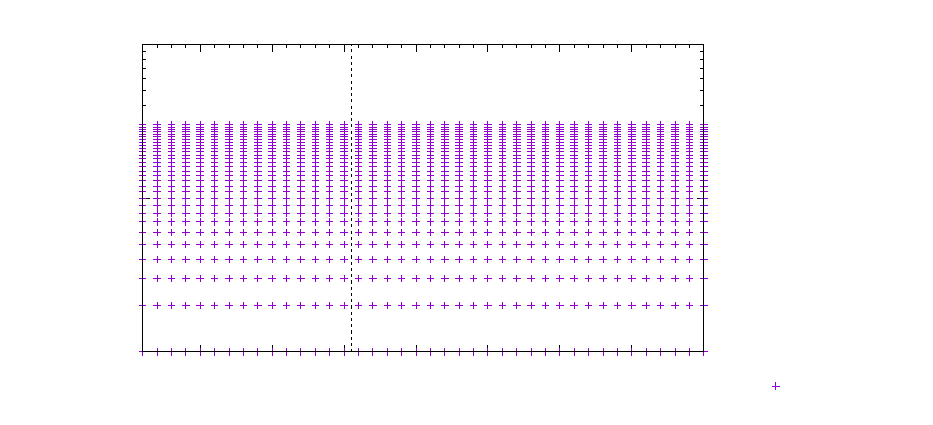
\includegraphics[width={432.00bp},height={188.60bp}]{../Plots/SCAMDWave/Diag/-2.5/plot}}%
    \gplfronttext
  \end{picture}%
\endgroup


    \caption{Progression of the complex phase of the gap in a 30 sites long SC for a range of chemical potentials.
     Phase on side $\varphi_0 = -2\pi/3$ and gradient of $117^{\circ}$.}
    \label{fig:Phase-2pi3}
\end{figure}
\begin{figure}[H]
    % GNUPLOT: LaTeX picture with Postscript
\begingroup
  % Encoding inside the plot.  In the header of your document, this encoding
  % should to defined, e.g., by using
  % \usepackage[cp1252,<other encodings>]{inputenc}
  \inputencoding{cp1252}%
  \makeatletter
  \providecommand\color[2][]{%
    \GenericError{(gnuplot) \space\space\space\@spaces}{%
      Package color not loaded in conjunction with
      terminal option `colourtext'%
    }{See the gnuplot documentation for explanation.%
    }{Either use 'blacktext' in gnuplot or load the package
      color.sty in LaTeX.}%
    \renewcommand\color[2][]{}%
  }%
  \providecommand\includegraphics[2][]{%
    \GenericError{(gnuplot) \space\space\space\@spaces}{%
      Package graphicx or graphics not loaded%
    }{See the gnuplot documentation for explanation.%
    }{The gnuplot epslatex terminal needs graphicx.sty or graphics.sty.}%
    \renewcommand\includegraphics[2][]{}%
  }%
  \providecommand\rotatebox[2]{#2}%
  \@ifundefined{ifGPcolor}{%
    \newif\ifGPcolor
    \GPcolortrue
  }{}%
  \@ifundefined{ifGPblacktext}{%
    \newif\ifGPblacktext
    \GPblacktextfalse
  }{}%
  % define a \g@addto@macro without @ in the name:
  \let\gplgaddtomacro\g@addto@macro
  % define empty templates for all commands taking text:
  \gdef\gplbacktext{}%
  \gdef\gplfronttext{}%
  \makeatother
  \ifGPblacktext
    % no textcolor at all
    \def\colorrgb#1{}%
    \def\colorgray#1{}%
  \else
    % gray or color?
    \ifGPcolor
      \def\colorrgb#1{\color[rgb]{#1}}%
      \def\colorgray#1{\color[gray]{#1}}%
      \expandafter\def\csname LTw\endcsname{\color{white}}%
      \expandafter\def\csname LTb\endcsname{\color{black}}%
      \expandafter\def\csname LTa\endcsname{\color{black}}%
      \expandafter\def\csname LT0\endcsname{\color[rgb]{1,0,0}}%
      \expandafter\def\csname LT1\endcsname{\color[rgb]{0,1,0}}%
      \expandafter\def\csname LT2\endcsname{\color[rgb]{0,0,1}}%
      \expandafter\def\csname LT3\endcsname{\color[rgb]{1,0,1}}%
      \expandafter\def\csname LT4\endcsname{\color[rgb]{0,1,1}}%
      \expandafter\def\csname LT5\endcsname{\color[rgb]{1,1,0}}%
      \expandafter\def\csname LT6\endcsname{\color[rgb]{0,0,0}}%
      \expandafter\def\csname LT7\endcsname{\color[rgb]{1,0.3,0}}%
      \expandafter\def\csname LT8\endcsname{\color[rgb]{0.5,0.5,0.5}}%
    \else
      % gray
      \def\colorrgb#1{\color{black}}%
      \def\colorgray#1{\color[gray]{#1}}%
      \expandafter\def\csname LTw\endcsname{\color{white}}%
      \expandafter\def\csname LTb\endcsname{\color{black}}%
      \expandafter\def\csname LTa\endcsname{\color{black}}%
      \expandafter\def\csname LT0\endcsname{\color{black}}%
      \expandafter\def\csname LT1\endcsname{\color{black}}%
      \expandafter\def\csname LT2\endcsname{\color{black}}%
      \expandafter\def\csname LT3\endcsname{\color{black}}%
      \expandafter\def\csname LT4\endcsname{\color{black}}%
      \expandafter\def\csname LT5\endcsname{\color{black}}%
      \expandafter\def\csname LT6\endcsname{\color{black}}%
      \expandafter\def\csname LT7\endcsname{\color{black}}%
      \expandafter\def\csname LT8\endcsname{\color{black}}%
    \fi
  \fi
    \setlength{\unitlength}{0.0500bp}%
    \ifx\gptboxheight\undefined%
      \newlength{\gptboxheight}%
      \newlength{\gptboxwidth}%
      \newsavebox{\gptboxtext}%
    \fi%
    \setlength{\fboxrule}{0.5pt}%
    \setlength{\fboxsep}{1pt}%
    \definecolor{tbcol}{rgb}{1,1,1}%
\begin{picture}(8640.00,3772.00)%
    \gplgaddtomacro\gplbacktext{%
      \csname LTb\endcsname%%
      \put(946,542){\makebox(0,0){\scriptsize 1}}%
      \put(946,2018){\makebox(0,0){\scriptsize 10}}%
      \put(946,3493){\makebox(0,0){\scriptsize 100}}%
      \put(1762,410){\makebox(0,0){\scriptsize 5}}%
      \put(2453,410){\makebox(0,0){\scriptsize 10}}%
      \put(3143,410){\makebox(0,0){\scriptsize 15}}%
      \put(3834,410){\makebox(0,0){\scriptsize 20}}%
      \put(4524,410){\makebox(0,0){\scriptsize 25}}%
      \put(5215,410){\makebox(0,0){\scriptsize 30}}%
      \put(5905,410){\makebox(0,0){\scriptsize 35}}%
      \put(6596,410){\makebox(0,0){\scriptsize 40}}%
      \put(2557,3670){\makebox(0,0){\strut{}SC}}%
      \put(5250,3670){\makebox(0,0){\strut{}AM}}%
    }%
    \gplgaddtomacro\gplfronttext{%
      \csname LTb\endcsname%%
      \put(7715,212){\makebox(0,0)[l]{\strut{}\footnotesize -2.5}}%
      \csname LTb\endcsname%%
      \put(605,2017){\rotatebox{-270.00}{\makebox(0,0){\strut{}$\bm{|\langle c_{i\uparrow}c_{i\downarrow}\rangle|$}}}}%
      \put(3903,212){\makebox(0,0){\small\textbf{Lattice site $i$ in $\bm{e}_x$}}}%
    }%
    \gplbacktext
    \put(0,0){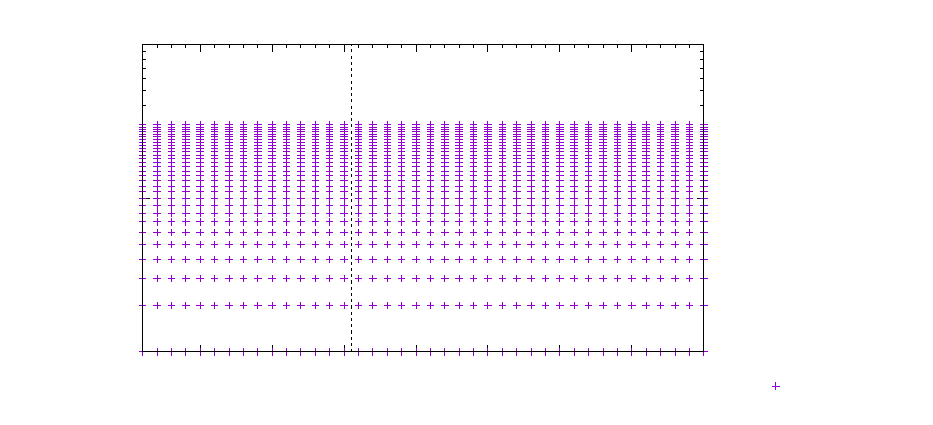
\includegraphics[width={432.00bp},height={188.60bp}]{../Plots/SCAMDWave/Diag/-2.5/plot}}%
    \gplfronttext
  \end{picture}%
\endgroup


    \caption{Complex phase of the gap in a 30 sites long SC. Phase on side $\varphi_0 = \pi/3$ and gradient of $117^{\circ}$.}
    \label{fig:Phasepi3}
\end{figure}
We see that the profile of the curve is the same regardless the starting phase. The slope of the gradient increase while lowering $|\mu|$.
Having the sides artificially fixed in the phase causes abrupt changes in the phase on the sides. We see however when skipping the first
 five sites from the edges, that the self-consistent
algorithm achieves to make a smooth transition. The Andrev bound states are still present and causes the small fluctuations we can see just after the
break.\\
\begin{figure}[H]
    % GNUPLOT: LaTeX picture with Postscript
\begingroup
  % Encoding inside the plot.  In the header of your document, this encoding
  % should to defined, e.g., by using
  % \usepackage[cp1252,<other encodings>]{inputenc}
  \inputencoding{cp1252}%
  \makeatletter
  \providecommand\color[2][]{%
    \GenericError{(gnuplot) \space\space\space\@spaces}{%
      Package color not loaded in conjunction with
      terminal option `colourtext'%
    }{See the gnuplot documentation for explanation.%
    }{Either use 'blacktext' in gnuplot or load the package
      color.sty in LaTeX.}%
    \renewcommand\color[2][]{}%
  }%
  \providecommand\includegraphics[2][]{%
    \GenericError{(gnuplot) \space\space\space\@spaces}{%
      Package graphicx or graphics not loaded%
    }{See the gnuplot documentation for explanation.%
    }{The gnuplot epslatex terminal needs graphicx.sty or graphics.sty.}%
    \renewcommand\includegraphics[2][]{}%
  }%
  \providecommand\rotatebox[2]{#2}%
  \@ifundefined{ifGPcolor}{%
    \newif\ifGPcolor
    \GPcolortrue
  }{}%
  \@ifundefined{ifGPblacktext}{%
    \newif\ifGPblacktext
    \GPblacktextfalse
  }{}%
  % define a \g@addto@macro without @ in the name:
  \let\gplgaddtomacro\g@addto@macro
  % define empty templates for all commands taking text:
  \gdef\gplbacktext{}%
  \gdef\gplfronttext{}%
  \makeatother
  \ifGPblacktext
    % no textcolor at all
    \def\colorrgb#1{}%
    \def\colorgray#1{}%
  \else
    % gray or color?
    \ifGPcolor
      \def\colorrgb#1{\color[rgb]{#1}}%
      \def\colorgray#1{\color[gray]{#1}}%
      \expandafter\def\csname LTw\endcsname{\color{white}}%
      \expandafter\def\csname LTb\endcsname{\color{black}}%
      \expandafter\def\csname LTa\endcsname{\color{black}}%
      \expandafter\def\csname LT0\endcsname{\color[rgb]{1,0,0}}%
      \expandafter\def\csname LT1\endcsname{\color[rgb]{0,1,0}}%
      \expandafter\def\csname LT2\endcsname{\color[rgb]{0,0,1}}%
      \expandafter\def\csname LT3\endcsname{\color[rgb]{1,0,1}}%
      \expandafter\def\csname LT4\endcsname{\color[rgb]{0,1,1}}%
      \expandafter\def\csname LT5\endcsname{\color[rgb]{1,1,0}}%
      \expandafter\def\csname LT6\endcsname{\color[rgb]{0,0,0}}%
      \expandafter\def\csname LT7\endcsname{\color[rgb]{1,0.3,0}}%
      \expandafter\def\csname LT8\endcsname{\color[rgb]{0.5,0.5,0.5}}%
    \else
      % gray
      \def\colorrgb#1{\color{black}}%
      \def\colorgray#1{\color[gray]{#1}}%
      \expandafter\def\csname LTw\endcsname{\color{white}}%
      \expandafter\def\csname LTb\endcsname{\color{black}}%
      \expandafter\def\csname LTa\endcsname{\color{black}}%
      \expandafter\def\csname LT0\endcsname{\color{black}}%
      \expandafter\def\csname LT1\endcsname{\color{black}}%
      \expandafter\def\csname LT2\endcsname{\color{black}}%
      \expandafter\def\csname LT3\endcsname{\color{black}}%
      \expandafter\def\csname LT4\endcsname{\color{black}}%
      \expandafter\def\csname LT5\endcsname{\color{black}}%
      \expandafter\def\csname LT6\endcsname{\color{black}}%
      \expandafter\def\csname LT7\endcsname{\color{black}}%
      \expandafter\def\csname LT8\endcsname{\color{black}}%
    \fi
  \fi
    \setlength{\unitlength}{0.0500bp}%
    \ifx\gptboxheight\undefined%
      \newlength{\gptboxheight}%
      \newlength{\gptboxwidth}%
      \newsavebox{\gptboxtext}%
    \fi%
    \setlength{\fboxrule}{0.5pt}%
    \setlength{\fboxsep}{1pt}%
    \definecolor{tbcol}{rgb}{1,1,1}%
\begin{picture}(8640.00,3772.00)%
    \gplgaddtomacro\gplbacktext{%
      \csname LTb\endcsname%%
      \put(946,542){\makebox(0,0){\scriptsize 1}}%
      \put(946,2018){\makebox(0,0){\scriptsize 10}}%
      \put(946,3493){\makebox(0,0){\scriptsize 100}}%
      \put(1762,410){\makebox(0,0){\scriptsize 5}}%
      \put(2453,410){\makebox(0,0){\scriptsize 10}}%
      \put(3143,410){\makebox(0,0){\scriptsize 15}}%
      \put(3834,410){\makebox(0,0){\scriptsize 20}}%
      \put(4524,410){\makebox(0,0){\scriptsize 25}}%
      \put(5215,410){\makebox(0,0){\scriptsize 30}}%
      \put(5905,410){\makebox(0,0){\scriptsize 35}}%
      \put(6596,410){\makebox(0,0){\scriptsize 40}}%
      \put(2557,3670){\makebox(0,0){\strut{}SC}}%
      \put(5250,3670){\makebox(0,0){\strut{}AM}}%
    }%
    \gplgaddtomacro\gplfronttext{%
      \csname LTb\endcsname%%
      \put(7715,212){\makebox(0,0)[l]{\strut{}\footnotesize -2.5}}%
      \csname LTb\endcsname%%
      \put(605,2017){\rotatebox{-270.00}{\makebox(0,0){\strut{}$\bm{|\langle c_{i\uparrow}c_{i\downarrow}\rangle|$}}}}%
      \put(3903,212){\makebox(0,0){\small\textbf{Lattice site $i$ in $\bm{e}_x$}}}%
    }%
    \gplbacktext
    \put(0,0){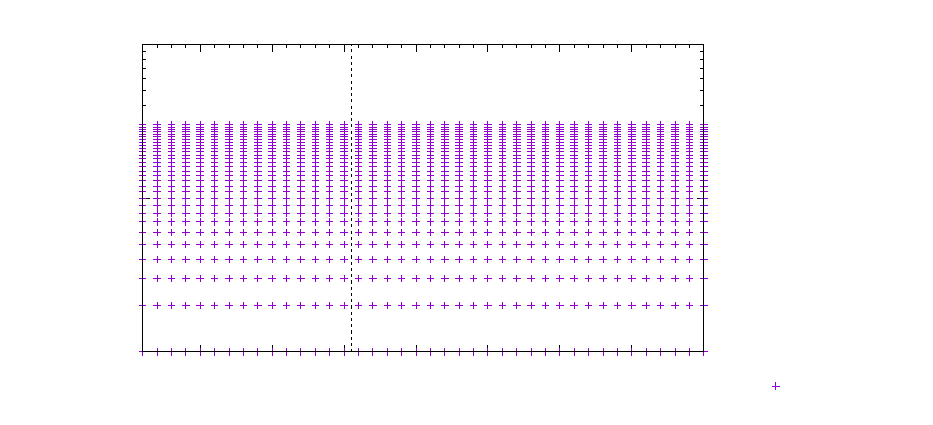
\includegraphics[width={432.00bp},height={188.60bp}]{../Plots/SCAMDWave/Diag/-2.5/plot}}%
    \gplfronttext
  \end{picture}%
\endgroup


    \caption{Current from a phase gradient of $117^{\circ}$ at $\mu = -1.75$.}
\end{figure}
\begin{figure}[H]
    % GNUPLOT: LaTeX picture with Postscript
\begingroup
  % Encoding inside the plot.  In the header of your document, this encoding
  % should to defined, e.g., by using
  % \usepackage[cp1252,<other encodings>]{inputenc}
  \inputencoding{cp1252}%
  \makeatletter
  \providecommand\color[2][]{%
    \GenericError{(gnuplot) \space\space\space\@spaces}{%
      Package color not loaded in conjunction with
      terminal option `colourtext'%
    }{See the gnuplot documentation for explanation.%
    }{Either use 'blacktext' in gnuplot or load the package
      color.sty in LaTeX.}%
    \renewcommand\color[2][]{}%
  }%
  \providecommand\includegraphics[2][]{%
    \GenericError{(gnuplot) \space\space\space\@spaces}{%
      Package graphicx or graphics not loaded%
    }{See the gnuplot documentation for explanation.%
    }{The gnuplot epslatex terminal needs graphicx.sty or graphics.sty.}%
    \renewcommand\includegraphics[2][]{}%
  }%
  \providecommand\rotatebox[2]{#2}%
  \@ifundefined{ifGPcolor}{%
    \newif\ifGPcolor
    \GPcolortrue
  }{}%
  \@ifundefined{ifGPblacktext}{%
    \newif\ifGPblacktext
    \GPblacktextfalse
  }{}%
  % define a \g@addto@macro without @ in the name:
  \let\gplgaddtomacro\g@addto@macro
  % define empty templates for all commands taking text:
  \gdef\gplbacktext{}%
  \gdef\gplfronttext{}%
  \makeatother
  \ifGPblacktext
    % no textcolor at all
    \def\colorrgb#1{}%
    \def\colorgray#1{}%
  \else
    % gray or color?
    \ifGPcolor
      \def\colorrgb#1{\color[rgb]{#1}}%
      \def\colorgray#1{\color[gray]{#1}}%
      \expandafter\def\csname LTw\endcsname{\color{white}}%
      \expandafter\def\csname LTb\endcsname{\color{black}}%
      \expandafter\def\csname LTa\endcsname{\color{black}}%
      \expandafter\def\csname LT0\endcsname{\color[rgb]{1,0,0}}%
      \expandafter\def\csname LT1\endcsname{\color[rgb]{0,1,0}}%
      \expandafter\def\csname LT2\endcsname{\color[rgb]{0,0,1}}%
      \expandafter\def\csname LT3\endcsname{\color[rgb]{1,0,1}}%
      \expandafter\def\csname LT4\endcsname{\color[rgb]{0,1,1}}%
      \expandafter\def\csname LT5\endcsname{\color[rgb]{1,1,0}}%
      \expandafter\def\csname LT6\endcsname{\color[rgb]{0,0,0}}%
      \expandafter\def\csname LT7\endcsname{\color[rgb]{1,0.3,0}}%
      \expandafter\def\csname LT8\endcsname{\color[rgb]{0.5,0.5,0.5}}%
    \else
      % gray
      \def\colorrgb#1{\color{black}}%
      \def\colorgray#1{\color[gray]{#1}}%
      \expandafter\def\csname LTw\endcsname{\color{white}}%
      \expandafter\def\csname LTb\endcsname{\color{black}}%
      \expandafter\def\csname LTa\endcsname{\color{black}}%
      \expandafter\def\csname LT0\endcsname{\color{black}}%
      \expandafter\def\csname LT1\endcsname{\color{black}}%
      \expandafter\def\csname LT2\endcsname{\color{black}}%
      \expandafter\def\csname LT3\endcsname{\color{black}}%
      \expandafter\def\csname LT4\endcsname{\color{black}}%
      \expandafter\def\csname LT5\endcsname{\color{black}}%
      \expandafter\def\csname LT6\endcsname{\color{black}}%
      \expandafter\def\csname LT7\endcsname{\color{black}}%
      \expandafter\def\csname LT8\endcsname{\color{black}}%
    \fi
  \fi
    \setlength{\unitlength}{0.0500bp}%
    \ifx\gptboxheight\undefined%
      \newlength{\gptboxheight}%
      \newlength{\gptboxwidth}%
      \newsavebox{\gptboxtext}%
    \fi%
    \setlength{\fboxrule}{0.5pt}%
    \setlength{\fboxsep}{1pt}%
    \definecolor{tbcol}{rgb}{1,1,1}%
\begin{picture}(8640.00,3772.00)%
    \gplgaddtomacro\gplbacktext{%
      \csname LTb\endcsname%%
      \put(946,542){\makebox(0,0){\scriptsize 1}}%
      \put(946,2018){\makebox(0,0){\scriptsize 10}}%
      \put(946,3493){\makebox(0,0){\scriptsize 100}}%
      \put(1762,410){\makebox(0,0){\scriptsize 5}}%
      \put(2453,410){\makebox(0,0){\scriptsize 10}}%
      \put(3143,410){\makebox(0,0){\scriptsize 15}}%
      \put(3834,410){\makebox(0,0){\scriptsize 20}}%
      \put(4524,410){\makebox(0,0){\scriptsize 25}}%
      \put(5215,410){\makebox(0,0){\scriptsize 30}}%
      \put(5905,410){\makebox(0,0){\scriptsize 35}}%
      \put(6596,410){\makebox(0,0){\scriptsize 40}}%
      \put(2557,3670){\makebox(0,0){\strut{}SC}}%
      \put(5250,3670){\makebox(0,0){\strut{}AM}}%
    }%
    \gplgaddtomacro\gplfronttext{%
      \csname LTb\endcsname%%
      \put(7715,212){\makebox(0,0)[l]{\strut{}\footnotesize -2.5}}%
      \csname LTb\endcsname%%
      \put(605,2017){\rotatebox{-270.00}{\makebox(0,0){\strut{}$\bm{|\langle c_{i\uparrow}c_{i\downarrow}\rangle|$}}}}%
      \put(3903,212){\makebox(0,0){\small\textbf{Lattice site $i$ in $\bm{e}_x$}}}%
    }%
    \gplbacktext
    \put(0,0){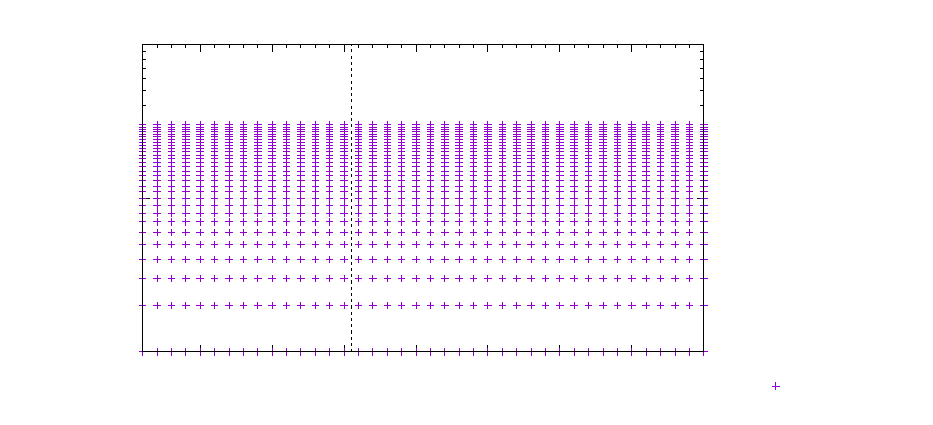
\includegraphics[width={432.00bp},height={188.60bp}]{../Plots/SCAMDWave/Diag/-2.5/plot}}%
    \gplfronttext
  \end{picture}%
\endgroup


    \caption{Current from a phase gradient of $117^{\circ}$ at $\mu = -2.75$.}
\end{figure}
\begin{figure}[H]
    % GNUPLOT: LaTeX picture with Postscript
\begingroup
  % Encoding inside the plot.  In the header of your document, this encoding
  % should to defined, e.g., by using
  % \usepackage[cp1252,<other encodings>]{inputenc}
  \inputencoding{cp1252}%
  \makeatletter
  \providecommand\color[2][]{%
    \GenericError{(gnuplot) \space\space\space\@spaces}{%
      Package color not loaded in conjunction with
      terminal option `colourtext'%
    }{See the gnuplot documentation for explanation.%
    }{Either use 'blacktext' in gnuplot or load the package
      color.sty in LaTeX.}%
    \renewcommand\color[2][]{}%
  }%
  \providecommand\includegraphics[2][]{%
    \GenericError{(gnuplot) \space\space\space\@spaces}{%
      Package graphicx or graphics not loaded%
    }{See the gnuplot documentation for explanation.%
    }{The gnuplot epslatex terminal needs graphicx.sty or graphics.sty.}%
    \renewcommand\includegraphics[2][]{}%
  }%
  \providecommand\rotatebox[2]{#2}%
  \@ifundefined{ifGPcolor}{%
    \newif\ifGPcolor
    \GPcolortrue
  }{}%
  \@ifundefined{ifGPblacktext}{%
    \newif\ifGPblacktext
    \GPblacktextfalse
  }{}%
  % define a \g@addto@macro without @ in the name:
  \let\gplgaddtomacro\g@addto@macro
  % define empty templates for all commands taking text:
  \gdef\gplbacktext{}%
  \gdef\gplfronttext{}%
  \makeatother
  \ifGPblacktext
    % no textcolor at all
    \def\colorrgb#1{}%
    \def\colorgray#1{}%
  \else
    % gray or color?
    \ifGPcolor
      \def\colorrgb#1{\color[rgb]{#1}}%
      \def\colorgray#1{\color[gray]{#1}}%
      \expandafter\def\csname LTw\endcsname{\color{white}}%
      \expandafter\def\csname LTb\endcsname{\color{black}}%
      \expandafter\def\csname LTa\endcsname{\color{black}}%
      \expandafter\def\csname LT0\endcsname{\color[rgb]{1,0,0}}%
      \expandafter\def\csname LT1\endcsname{\color[rgb]{0,1,0}}%
      \expandafter\def\csname LT2\endcsname{\color[rgb]{0,0,1}}%
      \expandafter\def\csname LT3\endcsname{\color[rgb]{1,0,1}}%
      \expandafter\def\csname LT4\endcsname{\color[rgb]{0,1,1}}%
      \expandafter\def\csname LT5\endcsname{\color[rgb]{1,1,0}}%
      \expandafter\def\csname LT6\endcsname{\color[rgb]{0,0,0}}%
      \expandafter\def\csname LT7\endcsname{\color[rgb]{1,0.3,0}}%
      \expandafter\def\csname LT8\endcsname{\color[rgb]{0.5,0.5,0.5}}%
    \else
      % gray
      \def\colorrgb#1{\color{black}}%
      \def\colorgray#1{\color[gray]{#1}}%
      \expandafter\def\csname LTw\endcsname{\color{white}}%
      \expandafter\def\csname LTb\endcsname{\color{black}}%
      \expandafter\def\csname LTa\endcsname{\color{black}}%
      \expandafter\def\csname LT0\endcsname{\color{black}}%
      \expandafter\def\csname LT1\endcsname{\color{black}}%
      \expandafter\def\csname LT2\endcsname{\color{black}}%
      \expandafter\def\csname LT3\endcsname{\color{black}}%
      \expandafter\def\csname LT4\endcsname{\color{black}}%
      \expandafter\def\csname LT5\endcsname{\color{black}}%
      \expandafter\def\csname LT6\endcsname{\color{black}}%
      \expandafter\def\csname LT7\endcsname{\color{black}}%
      \expandafter\def\csname LT8\endcsname{\color{black}}%
    \fi
  \fi
    \setlength{\unitlength}{0.0500bp}%
    \ifx\gptboxheight\undefined%
      \newlength{\gptboxheight}%
      \newlength{\gptboxwidth}%
      \newsavebox{\gptboxtext}%
    \fi%
    \setlength{\fboxrule}{0.5pt}%
    \setlength{\fboxsep}{1pt}%
    \definecolor{tbcol}{rgb}{1,1,1}%
\begin{picture}(8640.00,3772.00)%
    \gplgaddtomacro\gplbacktext{%
      \csname LTb\endcsname%%
      \put(946,542){\makebox(0,0){\scriptsize 1}}%
      \put(946,2018){\makebox(0,0){\scriptsize 10}}%
      \put(946,3493){\makebox(0,0){\scriptsize 100}}%
      \put(1762,410){\makebox(0,0){\scriptsize 5}}%
      \put(2453,410){\makebox(0,0){\scriptsize 10}}%
      \put(3143,410){\makebox(0,0){\scriptsize 15}}%
      \put(3834,410){\makebox(0,0){\scriptsize 20}}%
      \put(4524,410){\makebox(0,0){\scriptsize 25}}%
      \put(5215,410){\makebox(0,0){\scriptsize 30}}%
      \put(5905,410){\makebox(0,0){\scriptsize 35}}%
      \put(6596,410){\makebox(0,0){\scriptsize 40}}%
      \put(2557,3670){\makebox(0,0){\strut{}SC}}%
      \put(5250,3670){\makebox(0,0){\strut{}AM}}%
    }%
    \gplgaddtomacro\gplfronttext{%
      \csname LTb\endcsname%%
      \put(7715,212){\makebox(0,0)[l]{\strut{}\footnotesize -2.5}}%
      \csname LTb\endcsname%%
      \put(605,2017){\rotatebox{-270.00}{\makebox(0,0){\strut{}$\bm{|\langle c_{i\uparrow}c_{i\downarrow}\rangle|$}}}}%
      \put(3903,212){\makebox(0,0){\small\textbf{Lattice site $i$ in $\bm{e}_x$}}}%
    }%
    \gplbacktext
    \put(0,0){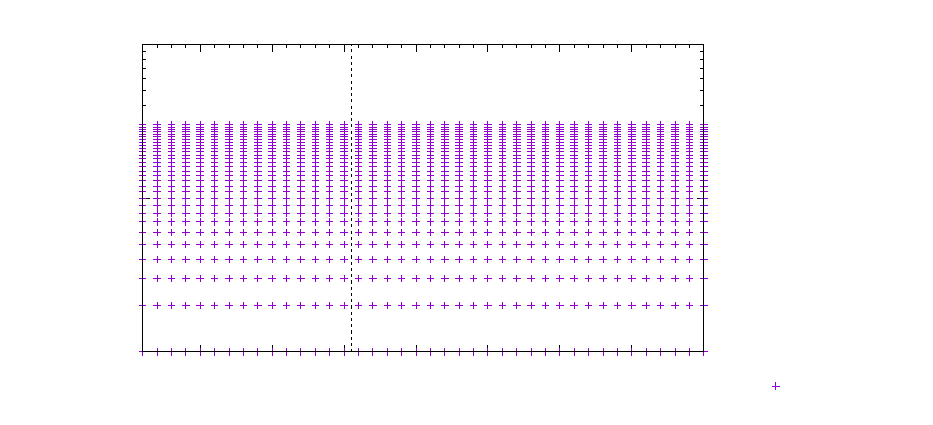
\includegraphics[width={432.00bp},height={188.60bp}]{../Plots/SCAMDWave/Diag/-2.5/plot}}%
    \gplfronttext
  \end{picture}%
\endgroup


    \caption{Current from a phase gradient of $117^{\circ}$ at $\mu = -3.75$.}
\end{figure}

\rem{Here the current varies along the $y$ direction but after the use of vertical boundary conditions we will have a uniform pattern.
We will skip the discussion of the current along the $y$ direction for now.}
We see that the current is very much related to the slope of the gradient, as it should be. 
The abrupt changes described in Fig. \ref{fig:Phase-2pi3} and \ref{fig:Phase-2pi3} causes low values in the current on the sides of the system. 
The current in the middle is ten times stronger with a $\mu$ of $-1.75$ than with a $\mu$ of $-2.75$. There are three orders of magnitude
of difference between the current strength in $\mu = -1.75$ and $-3.75$. The rule $I\propto\nabla\varphi$ is nevertheless verified.\\

One last check to make is the current continuity. No charges should be generated or lost. This of course doesn't apply on
the sides where we artificially fix the phase. Taking a function $f$ discretized on sites $i$ we have $\partial_x f = (f_{i+1} - f_{i-1} )/2a$,
$\partial_y f = (f_{i+N_x} - f_{i-N_x} )/2a$ with
$a$ the lattice spacing. We know that we normalized the lattice spacing to $1$. Finally, we have $\nabla f = (\partial_x + \partial_y) f$ as the divergence
of $f$.
\begin{figure}[H]
    % GNUPLOT: LaTeX picture with Postscript
\begingroup
  % Encoding inside the plot.  In the header of your document, this encoding
  % should to defined, e.g., by using
  % \usepackage[cp1252,<other encodings>]{inputenc}
  \inputencoding{cp1252}%
  \makeatletter
  \providecommand\color[2][]{%
    \GenericError{(gnuplot) \space\space\space\@spaces}{%
      Package color not loaded in conjunction with
      terminal option `colourtext'%
    }{See the gnuplot documentation for explanation.%
    }{Either use 'blacktext' in gnuplot or load the package
      color.sty in LaTeX.}%
    \renewcommand\color[2][]{}%
  }%
  \providecommand\includegraphics[2][]{%
    \GenericError{(gnuplot) \space\space\space\@spaces}{%
      Package graphicx or graphics not loaded%
    }{See the gnuplot documentation for explanation.%
    }{The gnuplot epslatex terminal needs graphicx.sty or graphics.sty.}%
    \renewcommand\includegraphics[2][]{}%
  }%
  \providecommand\rotatebox[2]{#2}%
  \@ifundefined{ifGPcolor}{%
    \newif\ifGPcolor
    \GPcolortrue
  }{}%
  \@ifundefined{ifGPblacktext}{%
    \newif\ifGPblacktext
    \GPblacktextfalse
  }{}%
  % define a \g@addto@macro without @ in the name:
  \let\gplgaddtomacro\g@addto@macro
  % define empty templates for all commands taking text:
  \gdef\gplbacktext{}%
  \gdef\gplfronttext{}%
  \makeatother
  \ifGPblacktext
    % no textcolor at all
    \def\colorrgb#1{}%
    \def\colorgray#1{}%
  \else
    % gray or color?
    \ifGPcolor
      \def\colorrgb#1{\color[rgb]{#1}}%
      \def\colorgray#1{\color[gray]{#1}}%
      \expandafter\def\csname LTw\endcsname{\color{white}}%
      \expandafter\def\csname LTb\endcsname{\color{black}}%
      \expandafter\def\csname LTa\endcsname{\color{black}}%
      \expandafter\def\csname LT0\endcsname{\color[rgb]{1,0,0}}%
      \expandafter\def\csname LT1\endcsname{\color[rgb]{0,1,0}}%
      \expandafter\def\csname LT2\endcsname{\color[rgb]{0,0,1}}%
      \expandafter\def\csname LT3\endcsname{\color[rgb]{1,0,1}}%
      \expandafter\def\csname LT4\endcsname{\color[rgb]{0,1,1}}%
      \expandafter\def\csname LT5\endcsname{\color[rgb]{1,1,0}}%
      \expandafter\def\csname LT6\endcsname{\color[rgb]{0,0,0}}%
      \expandafter\def\csname LT7\endcsname{\color[rgb]{1,0.3,0}}%
      \expandafter\def\csname LT8\endcsname{\color[rgb]{0.5,0.5,0.5}}%
    \else
      % gray
      \def\colorrgb#1{\color{black}}%
      \def\colorgray#1{\color[gray]{#1}}%
      \expandafter\def\csname LTw\endcsname{\color{white}}%
      \expandafter\def\csname LTb\endcsname{\color{black}}%
      \expandafter\def\csname LTa\endcsname{\color{black}}%
      \expandafter\def\csname LT0\endcsname{\color{black}}%
      \expandafter\def\csname LT1\endcsname{\color{black}}%
      \expandafter\def\csname LT2\endcsname{\color{black}}%
      \expandafter\def\csname LT3\endcsname{\color{black}}%
      \expandafter\def\csname LT4\endcsname{\color{black}}%
      \expandafter\def\csname LT5\endcsname{\color{black}}%
      \expandafter\def\csname LT6\endcsname{\color{black}}%
      \expandafter\def\csname LT7\endcsname{\color{black}}%
      \expandafter\def\csname LT8\endcsname{\color{black}}%
    \fi
  \fi
    \setlength{\unitlength}{0.0500bp}%
    \ifx\gptboxheight\undefined%
      \newlength{\gptboxheight}%
      \newlength{\gptboxwidth}%
      \newsavebox{\gptboxtext}%
    \fi%
    \setlength{\fboxrule}{0.5pt}%
    \setlength{\fboxsep}{1pt}%
    \definecolor{tbcol}{rgb}{1,1,1}%
\begin{picture}(8640.00,3772.00)%
    \gplgaddtomacro\gplbacktext{%
      \csname LTb\endcsname%%
      \put(946,542){\makebox(0,0){\scriptsize 1}}%
      \put(946,2018){\makebox(0,0){\scriptsize 10}}%
      \put(946,3493){\makebox(0,0){\scriptsize 100}}%
      \put(1762,410){\makebox(0,0){\scriptsize 5}}%
      \put(2453,410){\makebox(0,0){\scriptsize 10}}%
      \put(3143,410){\makebox(0,0){\scriptsize 15}}%
      \put(3834,410){\makebox(0,0){\scriptsize 20}}%
      \put(4524,410){\makebox(0,0){\scriptsize 25}}%
      \put(5215,410){\makebox(0,0){\scriptsize 30}}%
      \put(5905,410){\makebox(0,0){\scriptsize 35}}%
      \put(6596,410){\makebox(0,0){\scriptsize 40}}%
      \put(2557,3670){\makebox(0,0){\strut{}SC}}%
      \put(5250,3670){\makebox(0,0){\strut{}AM}}%
    }%
    \gplgaddtomacro\gplfronttext{%
      \csname LTb\endcsname%%
      \put(7715,212){\makebox(0,0)[l]{\strut{}\footnotesize -2.5}}%
      \csname LTb\endcsname%%
      \put(605,2017){\rotatebox{-270.00}{\makebox(0,0){\strut{}$\bm{|\langle c_{i\uparrow}c_{i\downarrow}\rangle|$}}}}%
      \put(3903,212){\makebox(0,0){\small\textbf{Lattice site $i$ in $\bm{e}_x$}}}%
    }%
    \gplbacktext
    \put(0,0){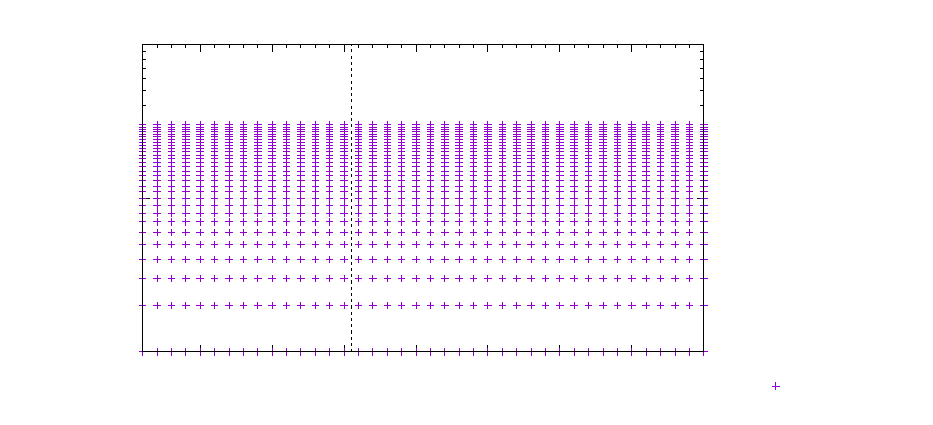
\includegraphics[width={432.00bp},height={188.60bp}]{../Plots/SCAMDWave/Diag/-2.5/plot}}%
    \gplfronttext
  \end{picture}%
\endgroup


    \caption{Continuity of the current from a phase gradient of $117^{\circ}$ at $\mu = -1.75$. In both $x$ and $y$ direction as
    well as the total continuity.}
\end{figure}
\begin{figure}[H]
    % GNUPLOT: LaTeX picture with Postscript
\begingroup
  % Encoding inside the plot.  In the header of your document, this encoding
  % should to defined, e.g., by using
  % \usepackage[cp1252,<other encodings>]{inputenc}
  \inputencoding{cp1252}%
  \makeatletter
  \providecommand\color[2][]{%
    \GenericError{(gnuplot) \space\space\space\@spaces}{%
      Package color not loaded in conjunction with
      terminal option `colourtext'%
    }{See the gnuplot documentation for explanation.%
    }{Either use 'blacktext' in gnuplot or load the package
      color.sty in LaTeX.}%
    \renewcommand\color[2][]{}%
  }%
  \providecommand\includegraphics[2][]{%
    \GenericError{(gnuplot) \space\space\space\@spaces}{%
      Package graphicx or graphics not loaded%
    }{See the gnuplot documentation for explanation.%
    }{The gnuplot epslatex terminal needs graphicx.sty or graphics.sty.}%
    \renewcommand\includegraphics[2][]{}%
  }%
  \providecommand\rotatebox[2]{#2}%
  \@ifundefined{ifGPcolor}{%
    \newif\ifGPcolor
    \GPcolortrue
  }{}%
  \@ifundefined{ifGPblacktext}{%
    \newif\ifGPblacktext
    \GPblacktextfalse
  }{}%
  % define a \g@addto@macro without @ in the name:
  \let\gplgaddtomacro\g@addto@macro
  % define empty templates for all commands taking text:
  \gdef\gplbacktext{}%
  \gdef\gplfronttext{}%
  \makeatother
  \ifGPblacktext
    % no textcolor at all
    \def\colorrgb#1{}%
    \def\colorgray#1{}%
  \else
    % gray or color?
    \ifGPcolor
      \def\colorrgb#1{\color[rgb]{#1}}%
      \def\colorgray#1{\color[gray]{#1}}%
      \expandafter\def\csname LTw\endcsname{\color{white}}%
      \expandafter\def\csname LTb\endcsname{\color{black}}%
      \expandafter\def\csname LTa\endcsname{\color{black}}%
      \expandafter\def\csname LT0\endcsname{\color[rgb]{1,0,0}}%
      \expandafter\def\csname LT1\endcsname{\color[rgb]{0,1,0}}%
      \expandafter\def\csname LT2\endcsname{\color[rgb]{0,0,1}}%
      \expandafter\def\csname LT3\endcsname{\color[rgb]{1,0,1}}%
      \expandafter\def\csname LT4\endcsname{\color[rgb]{0,1,1}}%
      \expandafter\def\csname LT5\endcsname{\color[rgb]{1,1,0}}%
      \expandafter\def\csname LT6\endcsname{\color[rgb]{0,0,0}}%
      \expandafter\def\csname LT7\endcsname{\color[rgb]{1,0.3,0}}%
      \expandafter\def\csname LT8\endcsname{\color[rgb]{0.5,0.5,0.5}}%
    \else
      % gray
      \def\colorrgb#1{\color{black}}%
      \def\colorgray#1{\color[gray]{#1}}%
      \expandafter\def\csname LTw\endcsname{\color{white}}%
      \expandafter\def\csname LTb\endcsname{\color{black}}%
      \expandafter\def\csname LTa\endcsname{\color{black}}%
      \expandafter\def\csname LT0\endcsname{\color{black}}%
      \expandafter\def\csname LT1\endcsname{\color{black}}%
      \expandafter\def\csname LT2\endcsname{\color{black}}%
      \expandafter\def\csname LT3\endcsname{\color{black}}%
      \expandafter\def\csname LT4\endcsname{\color{black}}%
      \expandafter\def\csname LT5\endcsname{\color{black}}%
      \expandafter\def\csname LT6\endcsname{\color{black}}%
      \expandafter\def\csname LT7\endcsname{\color{black}}%
      \expandafter\def\csname LT8\endcsname{\color{black}}%
    \fi
  \fi
    \setlength{\unitlength}{0.0500bp}%
    \ifx\gptboxheight\undefined%
      \newlength{\gptboxheight}%
      \newlength{\gptboxwidth}%
      \newsavebox{\gptboxtext}%
    \fi%
    \setlength{\fboxrule}{0.5pt}%
    \setlength{\fboxsep}{1pt}%
    \definecolor{tbcol}{rgb}{1,1,1}%
\begin{picture}(8640.00,3772.00)%
    \gplgaddtomacro\gplbacktext{%
      \csname LTb\endcsname%%
      \put(946,542){\makebox(0,0){\scriptsize 1}}%
      \put(946,2018){\makebox(0,0){\scriptsize 10}}%
      \put(946,3493){\makebox(0,0){\scriptsize 100}}%
      \put(1762,410){\makebox(0,0){\scriptsize 5}}%
      \put(2453,410){\makebox(0,0){\scriptsize 10}}%
      \put(3143,410){\makebox(0,0){\scriptsize 15}}%
      \put(3834,410){\makebox(0,0){\scriptsize 20}}%
      \put(4524,410){\makebox(0,0){\scriptsize 25}}%
      \put(5215,410){\makebox(0,0){\scriptsize 30}}%
      \put(5905,410){\makebox(0,0){\scriptsize 35}}%
      \put(6596,410){\makebox(0,0){\scriptsize 40}}%
      \put(2557,3670){\makebox(0,0){\strut{}SC}}%
      \put(5250,3670){\makebox(0,0){\strut{}AM}}%
    }%
    \gplgaddtomacro\gplfronttext{%
      \csname LTb\endcsname%%
      \put(7715,212){\makebox(0,0)[l]{\strut{}\footnotesize -2.5}}%
      \csname LTb\endcsname%%
      \put(605,2017){\rotatebox{-270.00}{\makebox(0,0){\strut{}$\bm{|\langle c_{i\uparrow}c_{i\downarrow}\rangle|$}}}}%
      \put(3903,212){\makebox(0,0){\small\textbf{Lattice site $i$ in $\bm{e}_x$}}}%
    }%
    \gplbacktext
    \put(0,0){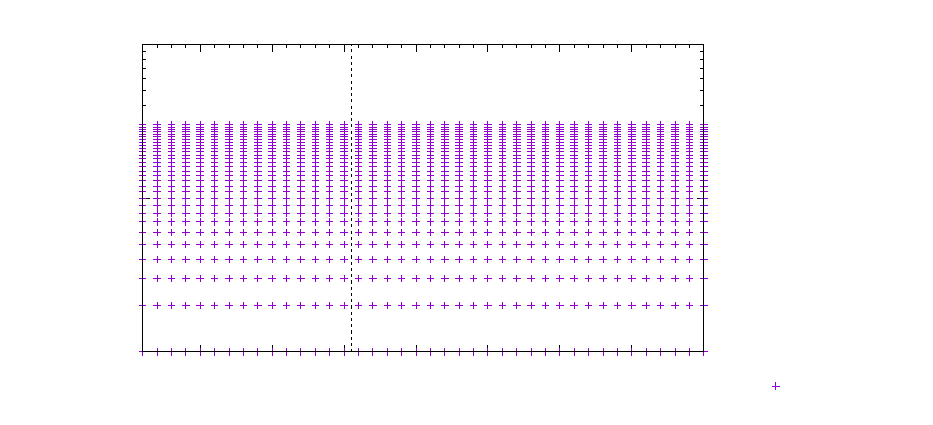
\includegraphics[width={432.00bp},height={188.60bp}]{../Plots/SCAMDWave/Diag/-2.5/plot}}%
    \gplfronttext
  \end{picture}%
\endgroup


    \caption{Continuity of the current from a phase gradient of $117^{\circ}$ at $\mu = -2.75$. In both $x$ and $y$ direction as
    well as the total continuity.}
\end{figure}
\begin{figure}[H]
    % GNUPLOT: LaTeX picture with Postscript
\begingroup
  % Encoding inside the plot.  In the header of your document, this encoding
  % should to defined, e.g., by using
  % \usepackage[cp1252,<other encodings>]{inputenc}
  \inputencoding{cp1252}%
  \makeatletter
  \providecommand\color[2][]{%
    \GenericError{(gnuplot) \space\space\space\@spaces}{%
      Package color not loaded in conjunction with
      terminal option `colourtext'%
    }{See the gnuplot documentation for explanation.%
    }{Either use 'blacktext' in gnuplot or load the package
      color.sty in LaTeX.}%
    \renewcommand\color[2][]{}%
  }%
  \providecommand\includegraphics[2][]{%
    \GenericError{(gnuplot) \space\space\space\@spaces}{%
      Package graphicx or graphics not loaded%
    }{See the gnuplot documentation for explanation.%
    }{The gnuplot epslatex terminal needs graphicx.sty or graphics.sty.}%
    \renewcommand\includegraphics[2][]{}%
  }%
  \providecommand\rotatebox[2]{#2}%
  \@ifundefined{ifGPcolor}{%
    \newif\ifGPcolor
    \GPcolortrue
  }{}%
  \@ifundefined{ifGPblacktext}{%
    \newif\ifGPblacktext
    \GPblacktextfalse
  }{}%
  % define a \g@addto@macro without @ in the name:
  \let\gplgaddtomacro\g@addto@macro
  % define empty templates for all commands taking text:
  \gdef\gplbacktext{}%
  \gdef\gplfronttext{}%
  \makeatother
  \ifGPblacktext
    % no textcolor at all
    \def\colorrgb#1{}%
    \def\colorgray#1{}%
  \else
    % gray or color?
    \ifGPcolor
      \def\colorrgb#1{\color[rgb]{#1}}%
      \def\colorgray#1{\color[gray]{#1}}%
      \expandafter\def\csname LTw\endcsname{\color{white}}%
      \expandafter\def\csname LTb\endcsname{\color{black}}%
      \expandafter\def\csname LTa\endcsname{\color{black}}%
      \expandafter\def\csname LT0\endcsname{\color[rgb]{1,0,0}}%
      \expandafter\def\csname LT1\endcsname{\color[rgb]{0,1,0}}%
      \expandafter\def\csname LT2\endcsname{\color[rgb]{0,0,1}}%
      \expandafter\def\csname LT3\endcsname{\color[rgb]{1,0,1}}%
      \expandafter\def\csname LT4\endcsname{\color[rgb]{0,1,1}}%
      \expandafter\def\csname LT5\endcsname{\color[rgb]{1,1,0}}%
      \expandafter\def\csname LT6\endcsname{\color[rgb]{0,0,0}}%
      \expandafter\def\csname LT7\endcsname{\color[rgb]{1,0.3,0}}%
      \expandafter\def\csname LT8\endcsname{\color[rgb]{0.5,0.5,0.5}}%
    \else
      % gray
      \def\colorrgb#1{\color{black}}%
      \def\colorgray#1{\color[gray]{#1}}%
      \expandafter\def\csname LTw\endcsname{\color{white}}%
      \expandafter\def\csname LTb\endcsname{\color{black}}%
      \expandafter\def\csname LTa\endcsname{\color{black}}%
      \expandafter\def\csname LT0\endcsname{\color{black}}%
      \expandafter\def\csname LT1\endcsname{\color{black}}%
      \expandafter\def\csname LT2\endcsname{\color{black}}%
      \expandafter\def\csname LT3\endcsname{\color{black}}%
      \expandafter\def\csname LT4\endcsname{\color{black}}%
      \expandafter\def\csname LT5\endcsname{\color{black}}%
      \expandafter\def\csname LT6\endcsname{\color{black}}%
      \expandafter\def\csname LT7\endcsname{\color{black}}%
      \expandafter\def\csname LT8\endcsname{\color{black}}%
    \fi
  \fi
    \setlength{\unitlength}{0.0500bp}%
    \ifx\gptboxheight\undefined%
      \newlength{\gptboxheight}%
      \newlength{\gptboxwidth}%
      \newsavebox{\gptboxtext}%
    \fi%
    \setlength{\fboxrule}{0.5pt}%
    \setlength{\fboxsep}{1pt}%
    \definecolor{tbcol}{rgb}{1,1,1}%
\begin{picture}(8640.00,3772.00)%
    \gplgaddtomacro\gplbacktext{%
      \csname LTb\endcsname%%
      \put(946,542){\makebox(0,0){\scriptsize 1}}%
      \put(946,2018){\makebox(0,0){\scriptsize 10}}%
      \put(946,3493){\makebox(0,0){\scriptsize 100}}%
      \put(1762,410){\makebox(0,0){\scriptsize 5}}%
      \put(2453,410){\makebox(0,0){\scriptsize 10}}%
      \put(3143,410){\makebox(0,0){\scriptsize 15}}%
      \put(3834,410){\makebox(0,0){\scriptsize 20}}%
      \put(4524,410){\makebox(0,0){\scriptsize 25}}%
      \put(5215,410){\makebox(0,0){\scriptsize 30}}%
      \put(5905,410){\makebox(0,0){\scriptsize 35}}%
      \put(6596,410){\makebox(0,0){\scriptsize 40}}%
      \put(2557,3670){\makebox(0,0){\strut{}SC}}%
      \put(5250,3670){\makebox(0,0){\strut{}AM}}%
    }%
    \gplgaddtomacro\gplfronttext{%
      \csname LTb\endcsname%%
      \put(7715,212){\makebox(0,0)[l]{\strut{}\footnotesize -2.5}}%
      \csname LTb\endcsname%%
      \put(605,2017){\rotatebox{-270.00}{\makebox(0,0){\strut{}$\bm{|\langle c_{i\uparrow}c_{i\downarrow}\rangle|$}}}}%
      \put(3903,212){\makebox(0,0){\small\textbf{Lattice site $i$ in $\bm{e}_x$}}}%
    }%
    \gplbacktext
    \put(0,0){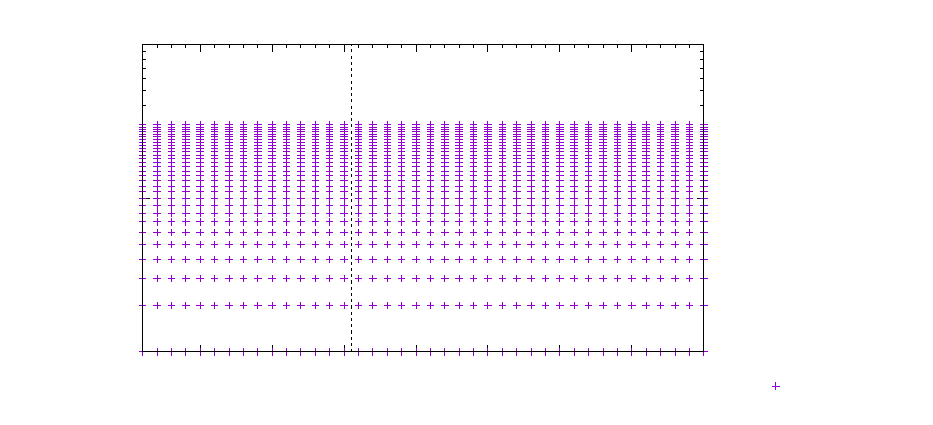
\includegraphics[width={432.00bp},height={188.60bp}]{../Plots/SCAMDWave/Diag/-2.5/plot}}%
    \gplfronttext
  \end{picture}%
\endgroup


    \caption{Continuity of the current from a phase gradient of $117^{\circ}$ at $\mu = -3.75$. In both $x$ and $y$ direction as
    well as the total continuity.}
\end{figure}
We see that the total discontinuity is always three orders of magnitude smaller than the current itself. This makes the discontinuity
significantly smaller than the current, and we can assume that this one is conserved. Once again a smaller convergence threshold
as well as an increase in the lattice definition would make the discontinuity even smaller.
We see that the $x$-component of the current is the one the less conserved. This fact is a direct result of the artificially fixed phased.

Far from the bulk, on the two first and last site, we observe cliff effects. This is due the abrupt changes in the phase we presented above.
The first cliff is positive, and the second one is negative.:
Considering the derivation we defined above, if the site $i+1$ has a stronger current than the site $i$, then $\partial_x I > 0$.
On the other hand for the last five sites we have $\partial_x I <0$ due to $I_{i+1}< I_i$. Here the current difference involved displays two to three orders of magnitude.
On the first and last site there is a discontinuity due to the missing neighbours. For the second and one before the last sites, there is a sudden change in the current
between sites two and three, as well as between the last and the one before the last site.\\
\rem{With the vertical periodic boundary condition we expect to have a uniform current along the $y$ direction.}




\subsection{Conclusion and outlook}
We have seen that the BCS superconducting gap is influenced by the Fermi surface. The gap is the largest when the Fermi surface is the largest.
The gap is also influenced by the presence of interfaces. We observe oscillations in the gap near the open boundaries, which are due to the reflection
of the quasiparticles with the sides.

Further we studied the leaking of the Cooper pairs in different materials. We observed an exponential decay in a normal metal.
This decay is modulated by oscillations that are due to the spin-dependent hopping in both the ferro- and altermagnet.
Due to the axis-dependence of the hopping, the oscillations are stronger in the altermagnet than in the ferromagnet.
Adding a diagonal interface to the system, we observed the same exponential decay and oscillations. The oscillations are more spread when considering
the leaking of the Cooper pairs along the normal of the interface. This is due to the interference of the leaking Cooper pairs.

Towards the modelling of a Josephon junction with an altermagnetic material, we achieved to represent the current in a superconductor.
The current is proportional with the phase gradient of the superconducting gap, and its strength grows with the number of Cooper pairs.
Moreover, the current verifies the charge conservation.
More work needs to be done to represent the current in the altermagnet between two different superconductors.\\

$d$-wave superconductivity was already introduced as being of particular interest. This is a more complex system.
As derived in the appendix, thegap is now a neighbour dependent quantity and is not isotropic in the momentum space. The goal would have been 
to study the profile of the gap when the Cooper pairs enter along the nodal lines of the gap geometry. This
would result is a clear difference when having a straight or diagonal interface. 
 Some work has been done towards studying the
proximity effect of a $d$-wave superconductor with the altermagnet. However, by lack of time we only achieved to represent the d-wave in a superconductor.



\begin{figure}[H]
    % GNUPLOT: LaTeX picture with Postscript
\begingroup
  % Encoding inside the plot.  In the header of your document, this encoding
  % should to defined, e.g., by using
  % \usepackage[cp1252,<other encodings>]{inputenc}
  \inputencoding{cp1252}%
  \makeatletter
  \providecommand\color[2][]{%
    \GenericError{(gnuplot) \space\space\space\@spaces}{%
      Package color not loaded in conjunction with
      terminal option `colourtext'%
    }{See the gnuplot documentation for explanation.%
    }{Either use 'blacktext' in gnuplot or load the package
      color.sty in LaTeX.}%
    \renewcommand\color[2][]{}%
  }%
  \providecommand\includegraphics[2][]{%
    \GenericError{(gnuplot) \space\space\space\@spaces}{%
      Package graphicx or graphics not loaded%
    }{See the gnuplot documentation for explanation.%
    }{The gnuplot epslatex terminal needs graphicx.sty or graphics.sty.}%
    \renewcommand\includegraphics[2][]{}%
  }%
  \providecommand\rotatebox[2]{#2}%
  \@ifundefined{ifGPcolor}{%
    \newif\ifGPcolor
    \GPcolortrue
  }{}%
  \@ifundefined{ifGPblacktext}{%
    \newif\ifGPblacktext
    \GPblacktextfalse
  }{}%
  % define a \g@addto@macro without @ in the name:
  \let\gplgaddtomacro\g@addto@macro
  % define empty templates for all commands taking text:
  \gdef\gplbacktext{}%
  \gdef\gplfronttext{}%
  \makeatother
  \ifGPblacktext
    % no textcolor at all
    \def\colorrgb#1{}%
    \def\colorgray#1{}%
  \else
    % gray or color?
    \ifGPcolor
      \def\colorrgb#1{\color[rgb]{#1}}%
      \def\colorgray#1{\color[gray]{#1}}%
      \expandafter\def\csname LTw\endcsname{\color{white}}%
      \expandafter\def\csname LTb\endcsname{\color{black}}%
      \expandafter\def\csname LTa\endcsname{\color{black}}%
      \expandafter\def\csname LT0\endcsname{\color[rgb]{1,0,0}}%
      \expandafter\def\csname LT1\endcsname{\color[rgb]{0,1,0}}%
      \expandafter\def\csname LT2\endcsname{\color[rgb]{0,0,1}}%
      \expandafter\def\csname LT3\endcsname{\color[rgb]{1,0,1}}%
      \expandafter\def\csname LT4\endcsname{\color[rgb]{0,1,1}}%
      \expandafter\def\csname LT5\endcsname{\color[rgb]{1,1,0}}%
      \expandafter\def\csname LT6\endcsname{\color[rgb]{0,0,0}}%
      \expandafter\def\csname LT7\endcsname{\color[rgb]{1,0.3,0}}%
      \expandafter\def\csname LT8\endcsname{\color[rgb]{0.5,0.5,0.5}}%
    \else
      % gray
      \def\colorrgb#1{\color{black}}%
      \def\colorgray#1{\color[gray]{#1}}%
      \expandafter\def\csname LTw\endcsname{\color{white}}%
      \expandafter\def\csname LTb\endcsname{\color{black}}%
      \expandafter\def\csname LTa\endcsname{\color{black}}%
      \expandafter\def\csname LT0\endcsname{\color{black}}%
      \expandafter\def\csname LT1\endcsname{\color{black}}%
      \expandafter\def\csname LT2\endcsname{\color{black}}%
      \expandafter\def\csname LT3\endcsname{\color{black}}%
      \expandafter\def\csname LT4\endcsname{\color{black}}%
      \expandafter\def\csname LT5\endcsname{\color{black}}%
      \expandafter\def\csname LT6\endcsname{\color{black}}%
      \expandafter\def\csname LT7\endcsname{\color{black}}%
      \expandafter\def\csname LT8\endcsname{\color{black}}%
    \fi
  \fi
    \setlength{\unitlength}{0.0500bp}%
    \ifx\gptboxheight\undefined%
      \newlength{\gptboxheight}%
      \newlength{\gptboxwidth}%
      \newsavebox{\gptboxtext}%
    \fi%
    \setlength{\fboxrule}{0.5pt}%
    \setlength{\fboxsep}{1pt}%
    \definecolor{tbcol}{rgb}{1,1,1}%
\begin{picture}(8640.00,3772.00)%
    \gplgaddtomacro\gplbacktext{%
      \csname LTb\endcsname%%
      \put(1122,1728){\makebox(0,0){\scriptsize 1e-06}}%
      \put(1122,2063){\makebox(0,0){\scriptsize 1e-05}}%
      \put(1122,2399){\makebox(0,0){\scriptsize 0.0001}}%
      \put(1122,2734){\makebox(0,0){\scriptsize 0.001}}%
      \put(1122,3069){\makebox(0,0){\scriptsize 0.01}}%
      \put(1122,3405){\makebox(0,0){\scriptsize 0.1}}%
      \put(1122,3740){\makebox(0,0){\scriptsize 1}}%
      \put(2092,1596){\makebox(0,0){\strut{}}}%
      \put(2975,1596){\makebox(0,0){\strut{}}}%
      \put(3858,1596){\makebox(0,0){\strut{}}}%
      \put(4741,1596){\makebox(0,0){\strut{}}}%
      \put(5624,1596){\makebox(0,0){\strut{}}}%
      \put(6507,1596){\makebox(0,0){\strut{}}}%
      \put(3947,3861){\makebox(0,0){\strut{}SC}}%
    }%
    \gplgaddtomacro\gplfronttext{%
      \csname LTb\endcsname%%
      \put(7626,2498){\makebox(0,0)[l]{\strut{}\footnotesize -3.75}}%
      \csname LTb\endcsname%%
      \put(7626,2278){\makebox(0,0)[l]{\strut{}\footnotesize -2.75}}%
      \csname LTb\endcsname%%
      \put(7626,2058){\makebox(0,0)[l]{\strut{}\footnotesize -1.75}}%
      \csname LTb\endcsname%%
      \put(7626,1838){\makebox(0,0)[l]{\strut{}\footnotesize -0.75}}%
      \csname LTb\endcsname%%
      \put(7626,1618){\makebox(0,0)[l]{\strut{}\footnotesize 0.75}}%
      \csname LTb\endcsname%%
      \put(7626,1398){\makebox(0,0)[l]{\strut{}\footnotesize 1.75}}%
      \csname LTb\endcsname%%
      \put(7626,1178){\makebox(0,0)[l]{\strut{}\footnotesize 2.75}}%
      \csname LTb\endcsname%%
      \put(7626,958){\makebox(0,0)[l]{\strut{}\footnotesize 3.75}}%
      \csname LTb\endcsname%%
      \put(253,2074){\rotatebox{-270.00}{\makebox(0,0){\strut{}$\bm{|F_d|}$}}}%
    }%
    \gplgaddtomacro\gplbacktext{%
      \csname LTb\endcsname%%
      \put(1115,843){\makebox(0,0){\scriptsize 1e-13}}%
      \put(1115,1383){\makebox(0,0){\scriptsize 1e-12}}%
      \put(2087,711){\makebox(0,0){ \(5\)}}%
      \put(2971,711){\makebox(0,0){ \(10\)}}%
      \put(3856,711){\makebox(0,0){ \(15\)}}%
      \put(4741,711){\makebox(0,0){ \(20\)}}%
      \put(5625,711){\makebox(0,0){ \(25\)}}%
      \put(6510,711){\makebox(0,0){ \(30\)}}%
    }%
    \gplgaddtomacro\gplfronttext{%
      \csname LTb\endcsname%%
      \put(3944,436){\makebox(0,0){\small\textbf{Lattice site $i$ in $\bm{e}_x$}}}%
    }%
    \gplbacktext
    \put(0,0){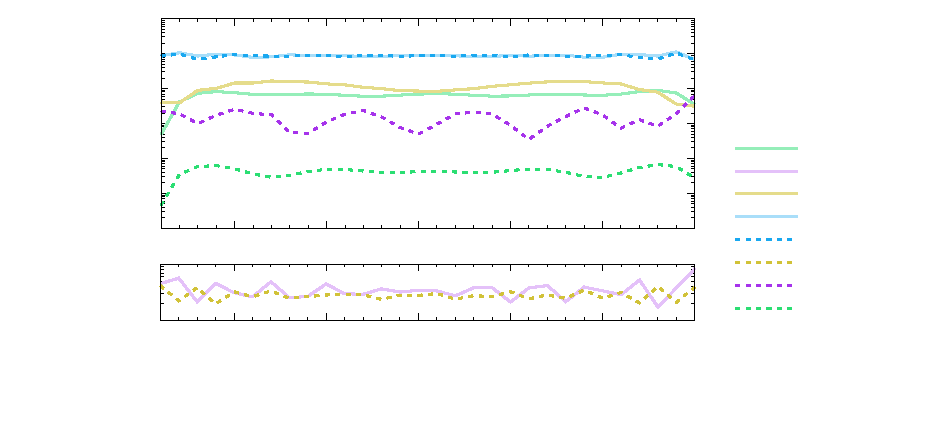
\includegraphics[width={432.00bp},height={188.60bp}]{../Plots/SC30/DWave/StraightInterface/FreeDelta/diffMUplot}}%
    \gplfronttext
  \end{picture}%
\endgroup


    \caption{$d$-wave superconductive parameter $F_d$ taking part into the gap $\Delta_{d,i} = V_i F_{d,i}$ for different chemical potential. This parameter is purely 
    real}
\end{figure}
As we can see the $d$-wave gap is not the same as the conventional BCS gap. We still observe this symmetry around $|\mu|$ for the range of selected chemical potentials in the bulk.
However, we have a decrease from $\pm3.5$ to $\pm2.5$ before growing towards $\pm0.5$. The parameter is weaker for $\mu=\pm2.5$ and $\pm3.5$ than the BCS gap but
about the same value for $\pm0.5$. We see that the Friedel oscillations as well as the presence of bound states still provoke oscillations on the sites near the vacuum.\\
We see as well that the gap is not symmetric around bulk along the $x$ axis. This might be caused by the oscillations that have different amplitude and frequency
for the different chemical potentials.\\


% \begin{tikzpicture}
%     \begin{axis}[
%         view={0}{90},  % Adjust the viewing angle
%         axis lines=center,
%         xlabel={$x$}, ylabel={$y$}, zlabel={$z$},
%         domain=-2*pi:2*pi, domain y=-2*pi:2*pi,
%         colormap/cool,
%       ]
%       % \addplot3[
%       %   surf,
%       %   shader=flat,
%       %   samples=50,
%       %   samples y=50,
%       %   z buffer=sort,
%       %   unbounded coords=jump,
%       % ]
%       % ({fd(x)},{y},{fd(x)}); % Using fd(x) for z-value

%       \addplot3[
%         surf,
%         shader=flat,
%         samples=100,
%         samples y=100,
%         z buffer=sort,
%         unbounded coords=jump,
%       ]
%       ({x},{y},{f(x,y,2)}); % Change th{f(x,y,0.5)}e last parameter (2) to set "a" \pgfmathifthenelse{abs(cos(x-pi) + cos(y-pi) - 2/2) < 1e-3}{2}{-2}}
%     \end{axis}
%   \end{tikzpicture}


\end{document}